\chapter{Limits of Sequences}
\begin{definition}{}{}
    A set $S$ is \textbf{closed under an operation}, $\circ$, (e.g., addition, multiplication, etc.) if, for any $a, b \in S$, the result of $a\circ b$ is also in $S$.
\end{definition}
\begin{example}{}{exp_3_0_1}
    \textcolor{red}{simple examples}
\end{example}



\section{Continuity of the Real Number System}
The understanding of number systems by humanity has been a progressive journey. Around $3000$ BCE, humans first recognized the natural number system $\mathbb{N}$, which is closed under addition and multiplication. By $2000$ BCE, with the development of trade and bookkeeping, the need to represent deficits and zero arose. It was realized that the natural number system is not closed under subtraction, leading to its extension to the integer set $\mathbb{Z}$. The integers are closed under addition, multiplication, and subtraction, but not under division. Around $500$ BCE, to meet the need for representing fractions, humanity extended the integers to the rational number set $\mathbb{Q}$. The set of rational numbers is closed under addition, subtraction, multiplication, and division (excluding division by zero). At this stage, rational numbers were considered sufficient, as they are closed under all four basic arithmetic operations. However, around $500$ BCE, the Pythagoreans in Ancient Greece discovered that $\mathbb{Q}$ is not closed under square root operations, as evidenced by the proof that $\sqrt{2} \not\in \mathbb{Q}$. 

\begin{example}{}{exp_3_1_1}
    Prove $\sqrt{2}$ is not rational.
    \begin{center}
        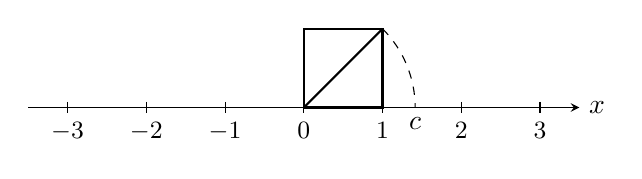
\begin{tikzpicture}[>=stealth]
            \draw[->] (-3.5,0) -- (3.5,0) node[right] {$x$};
            \foreach \x in {-3,-2,-1,0,1,2,3}
                \draw (\x,2pt) -- (\x,-2pt) node[below] {\small $\x$};
            \coordinate (Origin) at (0,0);
            \coordinate (BottomRight) at (1,0);
            \coordinate (TopRight) at (1,1);
            \coordinate (TopLeft) at (0,1);
            \draw[thick] (Origin) -- (BottomRight) -- (TopRight) -- (TopLeft) -- cycle;
            \draw[thick] (Origin) -- (TopRight);
            \draw[dashed] (1,1) arc (45:0:1.4142);
            \node[below] at (1.4142, 0) {$c$};
        \end{tikzpicture}
    \end{center}
\end{example}

\begin{proof}{MyExpColor}
    Let $c^{2} = 2$. For the purpose of contradiction, let $c \in \mathbb{Q}$ that is $c = \sqrt{2} = \frac{q}{p}, p, q \in \mathbb{N}$, and $p,q$ are coprime. Then $2 = \frac{q^{2}}{p^{2}} \iff 2p^{2} = q^{2}$. Since \textit{the square of an odd number is always odd}, we have that $q$ is even, which we assume to be $2k$. That is $q=2k, k\in \mathbb{N}$. Then we have $2 = \frac{4k^{2}}{p^{2}} \iff p^{2} = 2k^{2}$, that means $p$ is even as well. But if both $p$ and $q$ are even, this contradict the assumption that $p$ and $q$ are coprime. Therefore, $c=\sqrt{2}$ is not a rational number. In other words, the set of rational numbers is not closed under square root operations.
\end{proof}

\begin{note}
        The graph shows that The set of integers $\mathbb{Z}$ is \textbf{discrete} on the number line, whereas the set of rational numbers $\mathbb{Q}$ is \textbf{dense} on the number line but has \textbf{gaps} (i.e., $c$).
\end{note}

Later, in the $17$th century, Descartes introduced the concept of the real number line, and in the $19$th century, Dedekind and Cantor rigorously defined real numbers using methods such as Dedekind cuts and Cauchy sequences. This led to the construction of the real number system $\mathbb{R}$, which is closed under addition, subtraction, multiplication, division (excluding division by zero), square roots, and limits, thereby completing a significant milestone in the understanding of number systems.

\begin{definition}{}{def_3_1_1}
A \textbf{real number} is any number that can be represented on the number line. It includes all the rational and irrational numbers.
\[
\mathbb{R} = \left\{x \mid x \text{ is a rational or irrational number } \right\}.
\]
\end{definition}
\begin{note}
    The \textbf{continuity of real numbers} refers to the continuous distribution of elements in the real number set $\mathbb{R}$ on the number line, without any gaps or jumps.
\end{note}

\textbf{Question:} How do we know for sure that there is no gap in the set of real numbers?



\section{Infimum and Supremum}
Assume we have a finite set $S \subset \mathbb{R}$, $ S \neq \emptyset$, then the minimum and maximum of $S$ exist and are elements of $S$. However, if $S$ is an infinite set, it does not necessarily have a minimum or maximum. 

\textbf{Notation:} The symbol $\forall$ means "for any" or "for all". The symbol $\exists$ means "exists" or "we can find".

\begin{definition}{}{}
    We have a set $S \subset \mathbb{R}$, $ S \neq \emptyset$. If $\,\exists\, \xi \in S$ such that $\forall\, x \in S$, we have $x \leq \xi$, then $\xi$ is called a \textbf{maximum} of $S$, denoted $\max S$. If $\exists\, \eta \in S$ such that $\forall\, x \in S$, we have $ \eta \leq x$, then $\eta$ is called a \textbf{minimum} of $S$, denoted $\min S$.
\end{definition}

\begin{example}{}{}
    \textcolor{red}{Some simple examples}
\end{example}

\begin{example}{}{exp_3_2_2}
    Let $B = \{x \mid 0 \leq x < 1\}$, then show that $B$ does not have a maximum.
\end{example}
\begin{proof}{MyExpColor}
    We use prove by contradiction. Let $\beta \in B, \beta = \max B$, then $\beta \in [0, 1)$. Let $\beta^{\prime} = \frac{1+\beta}{2} \in B$. Since $\beta$ is the maximum, then we should have $\beta^{\prime} \leq \beta$, but obviously $\beta^{\prime} > \beta$.
\end{proof}


\begin{definition}{}{}
    Suppose we have a set $S \subset \mathbb{R}, S \neq \emptyset$. If $\exists\, M \in \textcolor{red}{\mathbb{R}}$, such that $\forall\, x \in S$, we have $x \leq M$, then $M$ is called \textcolor{red}{an} \textbf{upper bound} of $S$, or $S$ is \textbf{bounded above}. \textcolor{red}{(Here, since $M \in \mathbb{R}$, so there could be a lot of $M$.)}
\end{definition}

\begin{definition}{}{}
    Suppose $U$ is the set of all upper bounds of $S$, then $U$ does not have a maximum. But $U$ must have a minimum, (proof needed), denoted $\beta$. We say that $\beta$ is the \textbf{supremum} of $S$. That is $\beta = \sup S$. In other words, $\beta = \sup S$ conveys two idea:

    \begin{enumerate}[topsep=10pt, itemsep=5pt]
        \item $\sup S$ is an upper bound; that is $\forall\, x \in S$, we have $x \leq \beta$. 
        \item $\sup S$ is the smallest upper bound, that is $\forall\, \epsilon >0, \exists\, x \in S$ such that $x > \beta - \epsilon$.
    \end{enumerate}
\end{definition}

\begin{definition}{}{def_3_2_4}
    Suppose $L$ is the set of all lower bounds of $S$, then $L$ does not have a minimum. But $L$ must have a maximum, (proof needed), denoted $\alpha$. We say that $\alpha$ is the \textbf{infimum} of $S$. That is $\alpha = \inf S$. In other words, $\alpha = \inf S$ conveys two idea:
    
    \begin{enumerate}[topsep=10pt, itemsep=5pt]
        \item $\inf S$ is a lower bound; that is $\forall\, x \in S$, we have $x \geq \alpha$.
        \item $\inf S$ is the greatest lower bound; that is $\forall\, \epsilon >0, \exists\, x \in S$ such that $x < \alpha + \epsilon $.
     \end{enumerate}
\end{definition}



\subsection{Completeness Axiom}
\begin{theorem}{\quad Completeness Axiom / Least Upper Bounde Axiom / Supremum Property}{thm_3_2_1}
    Every non-empty subset of $\mathbb{R}$ that is bounded above has a supremum (least upper bound) in $\mathbb{R}$.
\end{theorem}

\begin{proof}{MyThmColor}
    Outline of the proof: 
    
    We treat every $x \in \mathbb{R}$ as the sum of its integer part, $\lfloor x \rfloor$, and its decimal part $(x)$. For the decimal part, we use $a_{i}, i \in \mathbb{N}$ to represent the $i$-th digit after the decimal point.  If $(x)$ is an infinite decimal, then it continues indefinitely. If $(x)$ is a finite decimal, then we assume it stops at the $p$-th digit after the decimal point, $a_{p} \neq 0$, then we add $0$ to the end of $a_{p}$. Then we using $0.999\dots = 1$ to get $(x) = 0.a_{1}a_{2}\dots a_{p}000\dots = 0.a_{1}a_{2}\dots (a_{p}-1)999\dots$.
    
    For all $x \in \mathbb{R}, \text{ We have } (x) = x - \lfloor x \rfloor \iff x = \lfloor x\rfloor + (x)$. That is
    
    \begin{enumerate}[topsep=10pt, itemsep=5pt]
        \item If $(x)$ is an infinite decimal, $(x) = 0.a_{1}a_{2}\dots a_{n}\dots$
        \item If $(x)$ is a finite decimal. W.L.O.G, we assume $(x)$ stops at, $a_{p} \neq 0$, the $p$-th digit after the decimal point, with $p \in \mathbb{N}$. That is $(x) = 0.a_{1}a_{2}\dots a_{p}000\dots = 0.a_{1}a_{2}\dots (a_{p}-1)999\dots$. (Here, we use the fact $0.\dot{9} = 1$.) 
    \end{enumerate}
    Assume there is an non-empty set $S \subseteq \mathbb{R}$, which is bounded above.
    \[
        S = \left\{ \textcolor{orange}{a_{0}} + \textcolor{blue}{0.a_{1}a_{2}\dots a_{n}\dots} \mid \textcolor{orange}{a_{0}} = \lfloor x\rfloor, \textcolor{blue}{0.a_{1}a_{2}\dots a_{n}\dots} = (x),\, x\in S  \right\}.
    \]
    Since $S$ is bounded above, we can find the largest $a_{0} = \lfloor x\rfloor$ in the $S$ and denote it as $\alpha_{0}$. Then we construct a new set $S_{0}$:
    \[
        S_{0} = \left\{ x \mid x \in S, \text{ and } \lfloor x\rfloor = \alpha_{0} \right\}.
    \]
    This means that all elements in $S_{0}$ have the largest units digit, $\alpha_{0}$. In other words, if $x \in S$ and $x \not\in S_{0}$ then $x < \alpha_{0}$. 
    
    Then, from elements in $S_{0}$, we choose the elements with the largest digit in the tenth place, and denote that largest tenth digit as $\alpha_{1}$. Then we construct another new set $S_{1}$:
    \[
        S_{1} = \left\{ x \mid x \in S_{0}, \text{ and the tenths place of } x \text{ is } \alpha_{1} \right\}.
    \]
    This means that if $x \in S$ and $X \not\in S_{1}$, then $x < \alpha_{0} + 0.\alpha_{1}$.
    
    We repeat this process by following the general rule, that is: From $S_{n-1}$, take the largest value of the $n$-th decimal place of the fractional part of $x \in S$, and denote it as $\alpha_{n}$. Then, we construct a new set $S_{n}$:
    \[
        S_{n} = \left\{ x \mid x \in S_{n-1} \text{ and the $n$-th decimal place of $x$ is } \alpha_{n} \right\}.
    \]
    Therefore, we have $S \subset S_{0} \subset S_{1} \subset S_{2} \subset \dots \subset S_{n} \subset \dots$. Since the latest set $S_{n}$ is built up on the previous set $S_{n-1}$, by picking fewer elements from $S_{n-1}$. (For elements from $S_{n-1}$, Only the elements with the largest $n$-th decimal place will be included in to $S_{n}$.) We also have $a_{0} \in \mathbb{Z}$ and $a_{1},a_{2}, \dots, a_{n},\dots \in \left\{0,1,2,\dots, 9\right\}$. 

    Let, $\beta = \alpha_{0} + 0.\alpha_{1}\alpha_{2}\dots\alpha_{n}\dots$. We just need to show that $\beta$ is the supremum of the set $S$.
    \begin{enumerate}
        \item[1)] We show $\beta$ is an upper bound. \\
        \textcolor{red}{For all $x\in S$, $x$ is either in $S$ but not in $S_{n}$, or $x$ in $S_{n}$.} If $x \in S, \text{ and } x \not\in S_{n}$, then $x < \alpha_{0} + 0.\alpha_{1}\alpha_{2}\dots\alpha_{n}000\dots \leq \beta$. If $x \in S_{n}, \forall\, n \in \mathbb{N}$, \textcolor{red}{we know not only the integer part of $x$ but also each decimal places of $x$ are the largest.} That is $x = \alpha_{0} + 0.\alpha_{1}\alpha_{2}\dots\alpha_{n}\dots = \beta$. Therefore, $\beta$ is an upper bound.
        \item[2)] We show that $\beta$ is the least upper bound. That is equivalent to find a small $\epsilon$ such that $\beta - \epsilon$ is not longer an upper bound. \\
        We pick $k \in \mathbb{N}$ such that $\epsilon > \frac{1}{10^{k}}$. Then choose $x \in S_{k}$, the integer part of this $x$ is $\alpha_{0}$, the first $k$ decimal parts this $x$ is $\alpha_{1},\alpha_{2},\dots,\alpha_{k}$. Then we have:
        \[
            \beta - x = \alpha_{0} + 0.\alpha_{1}\alpha_{2}\dots\alpha_{n}\dots - (\alpha_{0} + 0.\alpha_{1}\alpha_{2}\dots\alpha_{k}) \,\textcolor{red}{\leq}\, \frac{1}{10^{k}} < \epsilon \implies x > \beta -\epsilon.
        \]
        The red inequality is because the difference between $\beta$ and $x$ occurs after $\alpha_{k}$. For example, if $k=2$ then the largest difference between $\beta$ and $x$ could be $0.009$, while $\frac{1}{10^{2}} = 0.01$.Therefore, we have show $\beta$ is the least upper bound.    
    \end{enumerate}
    
    \indent Thus, we have shown that for any non-empty set $S \subset \mathbb{R}$ that is bounded above has a supremum.             
\end{proof}

Moreover, if the real number system has gaps (that is at some point, it is neither a rational number nor a irrational number), then the set to the left of that point has no supremum \textcolor{red}{(within the real number system)} and the set to the right of the point has no infimum \textcolor{red}{(within the real number system)}. \textbf{The Supremum Existence Theorem} shows that there are no gaps in the real number system.

\begin{proposition}{}{prop_3_2_2}
    Every non-empty subset of  $\mathbb{R}$ that is bounded below has an infimum (greatest lower bound) in $\mathbb{R}$.
\end{proposition}

\begin{proof}{MyPropColor}
    Just for fun, let's prove this with a new method. Let $A \in \mathbb{R}$ be bounded blow with lower bound $C$. Consider the set
    \[
        B = \left\{ -a \mid a \in A\right\}.
    \]
    For any $x \in B$ we have that $-x \in A$ and so $-x \geq C$. Then we have $x \leq -C$. Thus $B$ is bounded above and non-empty and so by the completeness axiom (we just proved) has a least upper bound $U$. If we let $L = -U$ then for all $a \in A$  and $-a \in B$ we have $-a \leq U \iff a \geq -U = L$. This shows that $L$ is a lower bound of $A$. We now show that $L$ is the least lower bound. Since $U$ is the least upper bound of the set $B$ we know that if we take a $y \in A$ with $y > L$, then $-y \in B$ with $-y < -L =U$. Thus $-y$ is not an upper bound for $B$ so we can find another element $b \in B$ such that $b > -y$. However, this means that $-b \in A$ and $-b < y$. So, $y$ cannot be a lower bound for $A$ (and we assumed $y > A$) so $L$ is the greatest lower bound for $A$.
\end{proof}

Though this proof is shorter, it stands on the proof of the completeness Axiom. The following example shows that $\mathbb{Q}$ has no completeness property.

\begin{example}{}{exp_3_2_3}
    Assume $T\left\{x \mid x \in \mathbb{Q}, x > 0, \text{ and } x^{2} < 2 \right\}$, then $T$ has no supremum in $\mathbb{Q}$.
\end{example}

\begin{proof}{MyExpColor}
    Assume $T$ has a supremum in $\mathbb{Q}$, denoted as $\sup T = \frac{n}{m}$, $m,n$ coprime and $m,n\in \mathbb{N}$. Then
    \[
        1 < \left(\frac{n}{m}\right)^{2} < 3
    \]
    Since $\frac{n}{m} \not\in \mathbb{Q}$, we have two situations:
    \begin{enumerate}
        \item[1).] $1 < \left(\frac{n}{m}\right)^{2} < 2$. We want to show that $\frac{n}{m}$ is not an upper bound. That is to find an $r >0, r \in \mathbb{Q}$, such that $\frac{n}{m} +r \in T$. In other words, we need to show $\left( \frac{n}{m} + r \right)^{2} < 2$. That is 
        \begin{align*}
            r^{2} + \frac{2n}{m}r + \left(\frac{n}{m}\right)^{2} &< 2 \\
            r^{2} + \frac{2n}{m}r + \underbrace{\frac{n^{2}}{m^{2}} -2}_{=-t} &< 0 \\
            \textcolor{blue}{r^{2} + \frac{2n}{m}r} -t &< 0. 
        \end{align*}
        Here, we let $t = 2 - \frac{n^{2}}{m^{2}}$, thus $t \in (0,1)$, for the purpose of applying $t^{2} < t$. We also have the inequality $1 < \frac{n^{2}}{m^{2}} < 2$. We observe the possible form for $r$ should be $r = \frac{an}{bm}t > 0, a,b,\in \mathbb{N}$. We substitute it into what we left to get
        \begin{align*}
            \textcolor{blue}{\frac{a^{2}n^{2}}{b^{2}m^{2}}t^{2} + \frac{2n^{2}}{bm^{2}}t} - t &< 0 \\
            \textcolor{blue}{\frac{a^{2}n^{2}}{b^{2}m^{2}}t^{2} + \frac{2n^{2}}{bm^{2}}t} &< t \\
        \end{align*}
        Since $t \in (0,1)$, then $\frac{a^{2}n^{2}}{b^{2}m^{2}}t^{2} < \frac{a^{2}n^{2}}{b^{2}m^{2}}t$, then we have 
        \begin{align*}
            \textcolor{blue}{\frac{a^{2}n^{2}}{b^{2}m^{2}}t + \frac{2n^{2}}{bm^{2}}t} < t
        \end{align*}
        We observe that as long as $\frac{a^{2}+2b}{b^{2}}\frac{n^{2}}{m^{2}} < 1$, the inequality above holds for sure. Since $\frac{n^{2}}{m^{2}} < 2$. We need to ensure $\frac{a^{2}+2b}{b^{2}} < \frac{1}{2}$. To keep it simple, we choose $a = 1 b = 5$ so that we let $r = \frac{n}{5m}t > 0$, this  will make $\left(\frac{n}{m} +r \right)^{2} < 2$, meaning $\frac{n}{m}$ is not an upper bound. Thus, contradiction. 
        \item[2).] $2 < \left(\frac{n}{m}\right)^{2} < 3$ We want to show that $\frac{n}{m}$ is not the least upper bound. That is to find an $r >0, r \in \mathbb{Q}$, such that $\frac{n}{m}-r$ is an upper bound. Let $\frac{n^{2}}{m^{2}}-2 = t$, then $t \in (0, 1)$. W.O.L.G.let $r = \frac{n}{5m}t > 0$. Obviously $\frac{n}{m} - t > 0 \text{ and } \frac{n}{m} - r \in \mathbb{Q}$. We also know that $\frac{2n}{m}r = \frac{2n^{2}}{5m^{2}}t < \frac{4}{5}t < t$. Therefor, 
        \[
        \left(\frac{n}{m} - r\right)^{2} -2 = r^{2} - \frac{2n}{m}r +t > 0.
        \]
        So, we have find a $r>0$ such that $\left(\frac{n}{m} - r\right)^{2}-2 >0 $, meaning that $\frac{n}{m}$ is not the lest upper bound. 

        Therefore, we have shown that $T$ has no supremum in $\mathbb{Q}$. In other words, $\mathbb{Q}$ has no completeness property.
    \end{enumerate}
\end{proof}

\begin{proposition}{Archimedean property}{prop_3_2_3}    
    For any $x \in \mathbb{R}$ there exists $k \in \mathbb{N}$ such that $k \geq x$.
\end{proposition}
\begin{proof}{MyPropColor}
    Fix $x \in \mathbb{R}$ and suppose that no such integer $k$ exists. This means that for all $z \in \mathbb{N}$ we have $z < x$ and so the natural numbers are bounded above by $x$. Thus by the completeness axiom the integers must have a least upper bound $\alpha$. Then $\alpha - \frac{1}{2}$ is not an upper bound for $\mathbb{N}$. So we can conclude that there is a natural number $z$ between $\alpha - \frac{1}{2}$ and $\alpha$. However, in this case $z+1$ is an integer greater than $\alpha$ and this contradicts with $alpha$ being the least upper bound.
\end{proof}



\section{Limits of Sequences}
A sequence is a function from a subset of the integers (usually the natural numbers) to a set. It is an ordered list of elements, where the order matters and repetition of elements is allowed. 
\[
    x_{1}, x_{2}, \dots, x_{n}, \dots
\]
\begin{definition}{}{}
    Formally, a \textbf{sequence} can be defined as: a function $f: \mathbb{N} \rightarrow X$, where $X$ is a set. The elements $a(n) = a_{n}$ are called the terms of the sequence, and $n \in \mathbb{N}$ represents their position in the sequence.
\end{definition}

\begin{example}{}{}
The following are some examples of sequences:
    \begin{align*}
        \left\{\frac{1}{n}\right\}&: \quad 1, \frac{1}{2}, \frac{1}{3}, \dots, \frac{1}{n},\dots. \\
        \left\{ (-1)^{n}\right\}&: 1, -1, 1, -1, \dots, (-1)^{n} \dots.
    \end{align*}
\end{example}

\begin{definition}{}{}
    \textbf{($\epsilon$-$N$ game)}.
    For a sequence $\{x_{n}\}$ and a real constant $A$. If for any \textcolor{red}{(given)} $\epsilon >0$ there exists an $N \in \mathbb{N}$ such that when $n > N$, we have $\vert x_{n} - a\vert < \epsilon$, then we say the sequence $\{x_{n}\}$ \textbf{converges} to $a$, denoted $\lim\limits_{n\rightarrow \infty} x_{n} = A$, or $x_{n} \overset{n \rightarrow \infty}{\longrightarrow} A$. If such an $A$ does not exist, then we say $\{x_{n}\}$ \textbf{diverges}. 
\end{definition}

\begin{note}
    The condition $\vert x_{n} -a\vert < \epsilon$ is equivalent to \textbf{the $\epsilon$ neighbourhood of point $A$}, denoted as $x_{n} \in O(A, \epsilon) = (A - \epsilon, A + \epsilon) = \left\{ x \mid A -\epsilon < x < A+\epsilon\right\}$.
\end{note}

\begin{remark}
    \textcolor{red}{Whether a sequence converges and, if so, to which value it converges, is independent of the first finitely many terms of the sequence.}
\end{remark}

\begin{example}{}{}
    \textcolor{red}{one simple example to address the remark.}   
\end{example}

\begin{example}{}{exp_3_3_3}
    Use the definite of limit of a sequence to show the limit of $\left\{\frac{n}{n+3}\right\}$ is $1$.
\end{example}

\begin{proof}{MyExpColor}
    For any \textcolor{red}{(given)} $\epsilon > 0$, we want $\vert\frac{n}{n+3} -1\vert < \epsilon \iff n > \frac{3}{\epsilon} - 3$. If we choose $N = \frac{3}{\epsilon} - 1$, we only need to ensure the RHS of is a positive integer. Since $\frac{3}{\epsilon} - 1 < \frac{3}{\epsilon}$ and to ensure it is an integer we choose $\lfloor\frac{3}{\epsilon} \rfloor$. To ensure it is positive (non-zero) we have $\lfloor\frac{3}{\epsilon} \rfloor < \lfloor\frac{3}{\epsilon} \rfloor + 1$. So, we choose $N = \lfloor\frac{3}{\epsilon} \rfloor + 1$. When $n > N$, we have $\vert\frac{n}{n+3} - 1 \vert < \epsilon$.
\end{proof}

\begin{remark}
    We enlarge the choice of $N$ several times to satisfy the condition for $N$.
\end{remark}

\begin{definition}{}{}
    A variable (in this case, a sequence) with $0$ as its limit is an \textbf{infinitesimal}.
\end{definition}

\begin{example}{}{}
    If $\lim\limits_{n \rightarrow \infty} x_{n} = a$ then immediately $x_{n} - a$ is an infinitesimal.    
\end{example}

\begin{example}{}{}
    Assume $0 < \vert q \vert < 1$ prove that $\left\{q^{n}\right\}$ is an infinitesimal.
\end{example}

\begin{proof}{MyExpColor}
    For any \textcolor{red}{(given)} $\epsilon > 0$, we have
    \begin{align*}
        \vert q^{n} -0 \vert  &< \epsilon \\
        \vert q^{n} \vert  &< \epsilon \\
        n\ln{\vert q\vert} < \ln{\epsilon} \\
        n > \frac{\ln{\epsilon}}{\ln{\vert q\vert }}.
    \end{align*}
Since $\ln{\vert q \vert}$ can be positive or negative, even with $\left\lfloor \frac{\ln{\epsilon}}{\ln{}\vert q\vert}\right\rfloor$, the positivity is not ensured so there is a trick to make sure it is positive. That is let $N = \max \left\{\left\lfloor\frac{\ln{\epsilon}}{\ln{\vert q \vert}}\right\rfloor, 1\right\}$, when $n > N$, we have $\vert q^{n} -0 \vert < \epsilon$.
\end{proof}

\begin{remark}
    When we are discussing something (i.e., a sequence) is getting very close to a value, it is obvious that we are talking about very small value of $\epsilon$. W.O.L.G., we often use $\epsilon \in (0,1)$ instead of $\epsilon > 0$. 
    
    For example, if we let $0 < \epsilon < \vert q\vert<1$, then $\frac{\ln{\epsilon}}{\ln{\vert q\vert}} > 1$. Then $N$ would be $\left\lfloor\frac{\ln{\epsilon}}{\ln{\vert q\vert}}\right\rfloor$. This tells us that if we restrict $\epsilon$ to a smaller interval, the choice of $N$ could be simpler. 

    \textcolor{red}{Suppose we have two students who find two different valid values of $N$, one being $100$ and another being $10000$. Which one is better? Both are correct answers, because in the definition of the limit, we only need to find an $N$ instead of the best (smallest) $N$. As we know to find the smallest (best) $N$ could sometimes be very challenging. Why make our life harder.} For example, in the inequality $n > RHS$, we often enlarge the RHS to make calculation easier, which leads to non-optimal but valid $N$.
\end{remark}

\begin{example}{}{}
    Prove $\lim\limits_{n \rightarrow \infty}\sqrt[n]{a} = 1$, for $(a > 1)$.
\end{example}

\begin{proof}{MyExpColor}
    \uwave{For any \textcolor{red}{(given)} $\epsilon > 0$}, let $\sqrt[n]{a} - 1= y_{n} >0$
    \begin{align*}
        \sqrt[n]{a} &= 1 + y_{n} \\
        a &= 1 + ny_{n} + \binom{n}{2}y_{n}^{2} + \dots + y^{n} \textcolor{red}{\, > \,} 1 + y_{n}^{n} \\
        y_{n} &< \frac{a-1}{n}
    \end{align*}
    We want to show $\left\vert \sqrt[n]{a} -1 \right\vert < \epsilon$ that is $ \sqrt[n]{a} -1 = y_{n}< \frac{a-1}{n} < \epsilon$. We easily got $n > \frac{a-1}{\epsilon}$. Thus, \uwave{we choose $N = \left\lfloor \frac{a-1}{\epsilon} \right\rfloor + 1$.} \uwave{When $n > N$, we have $\left\vert \sqrt[n]{a} -1 \right\vert = y_{n} < \frac{a-1}{n}< \epsilon$.}
\end{proof}

\begin{note}
    In the red inequality, we make the RHS smaller, since we do not need to find the best $N$. By doing so the proof is much easier.
\end{note}

For the previous example we do not need to use the method to make the RHS larger or smaller to solve the problem, but this is not true for the following example.

\begin{example}{}{exp_3_3_7}
    Show $\lim\limits_{n \to \infty}\sqrt[n]{n} = 1$.
\end{example}

\begin{proof}{MyExpColor}
    \uwave{For any \textcolor{red}{(given)} $\epsilon > 0$}, we want to show $\sqrt[n]{n} - 1 < \epsilon \iff \sqrt[n]{n} < 1+ \epsilon$. Let $\sqrt[n]{n} -1 = y_{n} > 0$ for $n = 2, 3, \dots$. Then we have
    \begin{align*}
        n = 1+ ny_{n} + \binom{n}{2}y_{n}^{2} + \dots + y_{n}^{n} &\textcolor{red}{\,>\,} 1 + \frac{n(n-1)}{2}y_{n}^{2} \\
        n &> 1 + \frac{n(n-1)}{2}y_{n}^{2} \\
        y_{n}^{2} &< \frac{2}{n} \\
        y_{n} &< \sqrt{\frac{2}{n}} < \epsilon \\
        n &> \frac{2}{\epsilon^{2}}.
    \end{align*}
    \uwave{We choose $N = \left\lfloor \frac{2}{\epsilon^{2}} \right\rfloor$,} \uwave{when $n > N$, we have $\left\vert \sqrt[n]{n} -1\right\vert < \epsilon$.}
\end{proof}

\begin{example}{}{}
    Prove $\lim\limits_{n \rightarrow \infty} \sqrt[n]{n^{2}} = 1$. 
\end{example}

\begin{proof}{MyExpColor}
     \textcolor{red}{We need $\binom{n}{3}y_{n}^{3}$}
\end{proof}

\begin{example}{}{}
    Prove $\lim\limits_{n \rightarrow \infty} \sqrt[n]{n^{k}} = 1$.
\end{example}

\begin{example}{}{}
    Prove $\lim\limits_{n \rightarrow \infty} \frac{n^{2}+1}{2n^{2}-7n} = \frac{1}{2}$.
\end{example}

\begin{proof}{MyExpColor}
    \uwave{For any \textcolor{red}{(given)} $\epsilon > 0$,} we want to show $\left\vert\frac{n^{2}}{2n^{2}-7n} 
- \frac{1}{2}\right\vert < \epsilon$. LHS is $\left\vert \frac{7n+2}{2n(2n-7)}\right\vert$, when $n > 3$ we get $\left\vert \frac{7n+2}{2n(2n-7)}\right\vert = \frac{7n+2}{2n(2n-7)} < \frac{8n}{2n(n-7)}$. This is still not simple enough. We keep enlarging it. That is $\frac{8n}{2n(n-7)} \textcolor{red}{\,<\,} \frac{8n}{4n^{2}}\cdot2 = \frac{4}{n}$. To ensure LHS $= \frac{7n+2}{2n(2n-7)} < \frac{4}{n}$, we got $n \geq 6$. Therefore, $\frac{4}{n} < \epsilon$, we get $n > \frac{4}{\epsilon}$. \uwave{We choose $N = \max\left\{\left\lfloor\frac{4}{\epsilon}\right\rfloor, 6\right\}$.} \uwave{When $n > N$, we have that $\left\vert\frac{n^{2}}{2n^{2}-7n} - \frac{1}{2}\right\vert < \epsilon$.}
\end{proof}

\begin{example}{}{}
    Suppose, $\lim\limits_{n \rightarrow \infty} a_{n} = a$, prove that $\lim\limits_{n \rightarrow \infty}\frac{a_{1} + a_{2} + \dots + a_{n}}{n} = a$.
\end{example}

\begin{proof}{MyExpColor}
    We discuss $a = 0$ and $a\neq 0$. 
    
    Case $1)$ 
    
    Suppose $a=0$. Since $\lim\limits_{n \rightarrow \infty} a_{n} = a$, that is \uwave{for any \textcolor{red}{(given)} $\epsilon > 0$,} \uwave{there exist $N_{1}$,} when $n > N_{1}$, $\vert a_{n}\vert < \frac{\epsilon}{2}$.
    \begin{align*}
        \frac{a_{1}+a_{2}+\dots + a_{n}}{n} &= \frac{a_{1}+a_{2}+\dots + a_{N_{1}}}{n} + \underbrace{\frac{a_{N_{1}+1}+a_{N_{1}+2}+\dots + a_{n}}{n}}_{\left\vert \frac{a_{N_{1}+1}+a_{N_{1}+2}+\dots + a_{n}}{n} \right\vert < \frac{(n - N_{1} + 1)+1}{n}\cdot\frac{\epsilon}{2} < \frac{\epsilon}{2}} \\
        \frac{a_{1}+a_{2}+\dots + a_{n}}{n} &< \textcolor{blue}{\frac{a_{1}+a_{2}+\dots + a_{N_{1}}}{n}} + \frac{\epsilon}{2}
    \end{align*}
    For the blue term, \textcolor{red}{since for a given $\epsilon$, $N_{1}$ is fixed, then $a_{1} + a_{2} + \dots + a_{N_{1}}$ is fixed}, then \uwave{we choose $N >> N_{1}$,} \uwave{such that when $n > N$,} we have $\left\vert \frac{a_{1}+ a_{2} + \dots + a_{N_{1}}}{n} \right\vert < \frac{\epsilon}{2}$. Therefore, we have $\frac{a_{1} + a_{2} + \dots + a_{n}}{n} < \epsilon$. 
    
    Case $2)$ 

    Suppose $a \neq 0$, then $a_{n} - a$ is an infinitesimal. We want to show 

    \begin{align*}
        &\lim\limits_{n \to \infty} \frac{a_{1} + a_{2} +\dots +a_{n}}{n} - a = 0 \\
        \quad \quad \quad &\text{or} \\
        &\left\vert \frac{a_{1} + a_{2} +\dots +a_{n}}{n} - a - 0 \right\vert < \epsilon
    \end{align*}
    W.O.L.G., we have  
    
    \begin{align*}
        \lim\limits_{n \rightarrow \infty} \frac{a_{1} + a_{2} +\dots +a_{n}}{n} - a = \lim_{n \rightarrow\infty }\frac{(a_{1}-a) + (a_{2}-a) + \dots + (a_{n}-a)}{n} \textcolor{red}{\,=\,} 0. 
    \end{align*}
    \textcolor{red}{The red equality is because now we view $(a_{n} - a)$ as new $a_{n}$ in case $1)$, so that we apply case $1)$ to get the answer.} Therefore, we have $\lim\limits_{n \rightarrow \infty}\frac{a_{1} + a_{2} + \dots + a_{n}}{n} = a$.
\end{proof}



\section{Properties of Limits of Sequences}
\begin{enumerate}
    \item [$1.$] \textbf{Uniqueness} of the limit of a sequence. 
    \begin{example}
        Suppose $\lim\limits_{n \rightarrow \infty} x_{n} = a$ and $\lim\limits_{n \rightarrow \infty} x_{n} = b$, then $a=b$.
    \end{example}
    
    \begin{proof}{MyExpColor}
        For $\lim\limits_{n \rightarrow \infty} x_{n} = a$, we have $\forall\, \epsilon > 0, \exists\, n >N_{1}$ such that $\left\vert x_{n} - a\right\vert < \frac{\epsilon}{2}$. For $\lim\limits_{n \rightarrow \infty} x_{n} = b$, we have $\forall\, \epsilon > 0, \exists n >N_{2}$ such that $\left\vert x_{n} - b\right\vert < \frac{\epsilon}{2}$. Therefore, we choose $N = \max\left\{N_{1}, N_{2}\right\}$, $\forall\, n > N$, $\left\vert a-b\right\vert \leq \left\vert x_{n} -a\right\vert + \left\vert x_{n}-b\right\vert < \epsilon$.
    \end{proof}

    \item [$2.$] \textbf{Convergent $\implies$ Bounded}. \\
    For a sequence $\left\{x_{n}\right\}$, if $\exists\, M \in \mathbb{R}, \forall\, n \in \mathbb{N}$ such that $x_{n} \leq M$, then $M$ is called an \textbf{upper bound} of the sequence $\left\{x_{n}\right\}$ or $\left\{x_{n}\right\}$ is \textbf{bounded above}. If $\exists\, m \in  \mathbb{R}, \forall\, n \in \mathbb{N}$ such that $x_{n} \geq m$, then $m$ is called a \textbf{lower bound} of the sequence $\left\{x_{n}\right\}$, or $\left\{x_{n}\right\}$ is \textbf{bounded below}. \\
    If $\left\{x_{n}\right\}$ has both upper bound and lower bound ($\vert x_{n} \vert \leq X, X \in \mathbb{R}^{+}$), then $\left\{x_{n}\right\}$ is a \textbf{bounded sequence}.

    \begin{theorem}{}{}
        A convergent sequence is always bounded.
    \end{theorem}

    \begin{proof}{MyThmColor}
        Suppose $\left\{x_{n}\right\}$ converges to $a$, that is for a \textcolor{red}{given} $\epsilon = 1$, there exists $N$, such that $\forall\, n > N$, we have $a-1 < x_{n} < a+1$. Now we only need to show the elements before $x_{N}$ are bounded. Let $M = \max\left\{x_{1},x _{2}, \dots, x_{N}, a+1\right\}$ and $m = \min\left\{x_{1}, x_{2}, \dots, x_{N}, a-1\right\}$ then we have $\forall\, n \in \mathbb{N}$, we have $m \leq x_{n} \leq M$.
    \end{proof}

    \item [$3.$] \textbf{Order Preservation} of limits of sequences.

    \begin{theorem}{}{thm_3_4_2}
        Suppose $\left\{x_{n}\right\}, \left\{y_{n}\right\}$ are two sequences and $\lim\limits_{n \rightarrow \infty}x_{n} = a, \lim\limits_{n \rightarrow \infty}x_{n} = b, a < b,$ then there exists $N \in \mathbb{N}$ such that $\forall\, n > N$, $x_{n} < y_{n}$.
        \begin{center}
            \begin{tikzpicture}[>=stealth, thick]
                \draw[->] (-4.5,0) -- (4.5,0);
                \filldraw ( -2,0) circle (1.5pt) node[below=5pt] {$a$};
                \filldraw (  2,0) circle (1.5pt) node[below=5pt] {$b$};
                \node at (-0.02,0) {$\boldsymbol{)}$};
                \node at (0.02,0) {$\boldsymbol{(}$};
                \draw[<-] (0,-0.2) -- (0,-1) node[below] {$\displaystyle \frac{a+b}{2}$};
                \node at (-3.5,0) {$\boldsymbol{(}$};
                \node at (3.5,0) {$\boldsymbol{)}$};
                \node[align=left] at (-4.5, 1) {$\{x_n\}$ \\ $\exists N_1, \forall n > N_1$};
                \node[align=left] at (4.5, 1) {$\{y_n\}$ \\ $\exists N_2, \forall n > N_2$};
                \draw[->] (-3, -0.6) node[below] {$x_n$} to [bend right=20] (-2, -0.6);
                \draw[->] (3, -0.6) node[below] {$y_n$} to [bend left=20] (2, -0.7);
            \end{tikzpicture}
        \end{center}
    \end{theorem}

    \begin{proof}{MyThmColor}
        We choose a \textcolor{red}{(given)} $\epsilon = \frac{b-a}{2} > 0$, there exists $N_{1} \in \mathbb{N}$ such that if $\forall\, n > N_{1}$ then $\left\vert x_{n} - a\right\vert < \epsilon \implies x_{n} < \frac{a+b}{2}$. There exists $N_{2} \in \mathbb{N}$ such that if $\forall\, n > N_{2}$ then $\left\vert y_{n} - b\right\vert < \epsilon \impliedby y_{n} > \frac{a+b}{2}$. Then we can choose $N = \max\left\{N_{1}, N_{2}\right\}$ such that if $n > N$ then $x_{x} < \frac{a+b}{2} < y_{n}$.
    \end{proof}  

    \begin{note}
        It is obvious that the limit of $\left\{x_{n}\right\}$ ensure that for very large $n$, $x_{n}$ will be in the neighborhood of $a$, $(a- \frac{b-a}{2}, a+\frac{b-a}{2})$. Similarly, for very large value of $n$, $y_{n}$ will be in the neighborhood of $b$, $(b- \frac{b-a}{2}, b+\frac{b-a}{2})$. In the graph it is clear that $x_{n} < y_{n}$.
    \end{note}

    \begin{remark}
        The converse is not true. That is $\lim\limits_{n \rightarrow \infty} x_{n} = a, \lim\limits_{n \rightarrow \infty} y_{n} = b, x_{n} < y_{n} \centernot\implies a < b$. For example, $x_{n} = \frac{1}{n}, y_{n} = \frac{2}{n}$, indeed $x_{n} < y_{n}, \forall\, n \in \mathbb{N}$, but $\lim\limits_{n \rightarrow \infty} x_{n} = \lim\limits_{n \rightarrow \infty} y_{n} = 0$. Actually we can only ensure that $a \textcolor{red}{\,\leq\,}b$ and the condition can be relaxed to $x_{n} \textcolor{red}{\,\leq\,} y_{n}$ for large value of $n$. This is the following proposition.
    \end{remark}

    \begin{proposition}{}{}
        Suppose $\lim\limits_{n \rightarrow \infty} x_{n} = a$, $\lim\limits_{n \rightarrow \infty} y_{n} = b$, if $\exists\, n > N$ such that $x_{n} \textcolor{red}{\,\leq\,} y_{n}$, then $a \textcolor{red}{\,\leq\,}b$.
    \end{proposition}

    \begin{corollary}{}{}
        Suppose $\lim\limits_{n \rightarrow \infty} y_{n} = b > 0$, then $\exists\, N$ such that $\forall\, n > N$ we have $y_{n} > \frac{b}{2} > 0$. [A certain distance to the right of the origin.] \textcolor{red}{similar graph} \textcolor{blue}{To prove this we need two sequences to use order preservation theorem, then we let $\left\{x_{n}\right\}$ be a sequence of constants with value $\frac{b}{2}$.}
    \end{corollary}

    \begin{corollary}{}{}
        Suppose $\lim\limits_{n \rightarrow \infty} y_{n} = b < 0$, then $\exists\, N$ such that $\forall\, n > N$ we have $y_{n} < \frac{b}{2} < 0$. [A certain distance to the left of the origin.] \textcolor{red}{similar graph}
    \end{corollary}

    \begin{corollary}{}{}
        Suppose $\lim\limits_{n \rightarrow \infty} y_{n} \neq 0$, then $\exists\, N$ such that $\forall\, n > N$ we have $\vert y_{n}\vert > \frac{\vert b\vert}{2} > 0$. [A certain distance from the origin.] \textcolor{red}{similar graph}
    \end{corollary}

    \item [$4.$] The \textbf{squeeze theorem}
    
    \begin{theorem}{}{}
         Suppose we have three sequences $\left\{x_{n}\right\}, \left\{y_{n}\right\}, \left\{z_{n}\right\}$. If $\exists\, N$, when $n > N$ such that $x_{n} \leq y_{n} \leq z_{n}$ and $\lim\limits_{n \rightarrow \infty}x_{n} = \lim\limits_{n \rightarrow \infty}z_{n} = a$, then $\lim\limits_{n \rightarrow \infty}y_{n} = a$.
    \end{theorem}

    \begin{proof}{MyThmColor}
        Since $\lim\limits_{n \rightarrow \infty}x_{n} = a$, \uwave{for a \textcolor{red}{(given)} $\epsilon$,} there exists $N_{1}\in \mathbb{N}$ such that when $n > N_{1}$, we have $\left\vert x_{n} - a \right\vert < \epsilon$. That is $a-\epsilon < x_{n}$. Similarly, for the same \textcolor{red}{(given)} $\epsilon$, since $\lim\limits_{n \rightarrow \infty}z_{n} = a$, there exists $N_{2}\in \mathbb{N}$ such that when $n > N_{2}$, we have $\left\vert z_{n} - a \right\vert < \epsilon$. That is $z_{n} < a + \epsilon$. Now \uwave{we choose $N = \max\left\{N_{1}, N_{2}\right\}$,} \uwave{when $n > N$,} we have $a - \epsilon < x_{n} \leq y_{n} \leq z_{n} < a+\epsilon$. That is \uwave{$a - \epsilon < y_{n} <  a+\epsilon \iff \left\vert y_{n} - a\right\vert < \epsilon$}. Therefore $\lim\limits_{n\rightarrow\infty}y_{n}=a$.
    \end{proof}
    \begin{example}{}{}
        Compute $\lim\limits_{n \rightarrow \infty} \left(\sqrt{n+1} - \sqrt{n}\right)$.
    \end{example}
    W.O.L.G., we have $0 < \sqrt{n+1} - \sqrt{n} = \frac{1}{\sqrt{n+1}+\sqrt{n}} < \frac{1}{\sqrt{n}}$. Since $\lim\limits_{n \rightarrow \infty} \frac{1}{\sqrt{n}} = 0$, then by the squeeze theorem, we have $\lim\limits_{n\rightarrow \infty} \left(\sqrt{n+1} - \sqrt{n}\right) = 0$.

    \begin{example}{}{}
        Proof that if $a_{1}, a_{2}, \dots, a_{p} > 0$ $\lim\limits_{n \rightarrow \infty}\left(a_{1}^{n} + a_{2}^{n} + \dots + a_{p}^{n} \right)^{\frac{1}{n}} = \max\limits_{1\leq i \leq p} \left\{a_{i}\right\}$.
    \end{example}
    \begin{proof}{MyExpColor}
        W.O.L.G., let's assume that $a_{1} = \max\limits_{1\leq i \leq p}\left\{a_{i}\right\}$. Then we have 
        \[ 
        a_{1} = \left(a_{1}^{n}\right)^{\frac{1}{n}} \leq \left(a_{1}^{n} + a_{2}^{n} + \dots + a_{p}^{n}\right)^{\frac{1}{n}} \leq \left(pa_{1}^{n}\right)^{\frac{1}{n}} = a_{1}p^{\frac{1}{n}}. 
        \]
        Recall that we have shown $a > 1, \lim\limits_{n \rightarrow \infty}\sqrt[n]{a} = 1$, then it is obvious that $p \geq 1$. Therefore, by the squeeze theorem, we have $\lim\limits_{n \rightarrow \infty}\left(a_{1}^{n} + a_{2}^{n} + \dots + a_{p}^{n} \right)^{\frac{1}{n}} = a_{1} = \max\limits_{1\leq i \leq p} \left\{a_{i}\right\}$.
    \end{proof}
    
    \begin{example}{}{}
        Prove $\lim\limits_{n\rightarrow \infty} \sqrt[n]{n}=1$.        
    \end{example}
    \begin{proof}{MyExpColor}
        Since $1 < \sqrt[n]{n} = \sqrt[n]{\sqrt{n}\cdot\sqrt{n}\cdot\underbrace{1\cdot1\dots1}_{n-2}} \textcolor{red}{\,\leq\,} \frac{2\sqrt{n} + n-2}{n} = 1 + \frac{2\sqrt{n}-2}{n}$. Since $\lim\limits_{n \rightarrow \infty} \frac{2\sqrt{n}-2}{n}=0$ and the squeeze theorem We have the proof. (The red inequality is due to the geometric mean is less than or equal to the arithmetic mean.)
    \end{proof}
    \begin{example}{}{}
        Prove $\lim\limits_{n\rightarrow \infty} \sqrt[n]{n^{2}}=1$.
    \end{example}
    \begin{proof}{MyExpColor}
        Since $1 < \sqrt[n]{n} = \sqrt[n]{\sqrt{n}\cdot\sqrt{n}\sqrt{n}\cdot\sqrt{n}\cdot\underbrace{1\cdot1\dots1}_{n-4}} \textcolor{red}{\,\leq\,} \frac{4\sqrt{n} + n-4}{n} = 1 + \frac{4\sqrt{n}-4}{n}$. Since $\lim\limits_{n \rightarrow \infty} \frac{4\sqrt{n}-4}{n}=0$ and the squeeze theorem We have the proof.
    \end{proof}
\end{enumerate}

\section{Arithmetic operations on the limits of sequences}
We start by stating the theorem.
\begin{theorem}{\quad}{thm_3_5_1}
    Suppose $\lim\limits_{n \rightarrow \infty} x_{n} = a, \lim\limits_{n\rightarrow \infty}y_{n}=b$, then we have 

    \begin{enumerate}[topsep=10pt, itemsep=5pt]
        \item $\lim\limits_{n \rightarrow \infty} \left(\alpha x_{n} + \beta y_{n}\right) = \alpha a + \beta b$; $\alpha, \beta$ are constants.
        \item $\lim\limits_{n\rightarrow \infty}\left(x_{n}y_{n}\right) = ab;$
        \item $\lim\limits_{n \rightarrow \infty} \frac{x_{n}}{y_{n}} = \frac{a}{b}, (b \neq 0).$ 
    \end{enumerate}
    \begin{note}
        In $3.$, $b\neq0$ ensures that when $n$ is large enough, all $y_{n}$ will be at some distance from zero. Although some early terms of the sequence $\left\{y_{n}\right\}$ can be zero, but for large $n$, this is not the case.
    \end{note}
\end{theorem}
\begin{proof}{MyThmColor}
    Since $\lim\limits_{n\rightarrow \infty }x_{n} = a$, then the sequence $\left\{x_{n}\right\}$ is bounded, that is $\exists\, X >0$ such that $\left\vert x_{n}\right\vert < X, \forall\, n \in \mathbb{N}$. Also, we have 
    \begin{align*}
        \uwave{\forall, \epsilon >0}, &\,\exists\, N_{1}, \forall\, n > N_{1} \text{ such that } \left\vert x_{n}-a\right\vert < \epsilon \\
                              &\,\exists\, N_{2}, \forall\, n > N_{2} \text{ such that } \left\vert y_{n}-b\right\vert < \epsilon
    \end{align*}
    \uwave{let $N = \max\left\{N_{1},N_{2}\right\}, \forall\, n > N$} we have
    \begin{align*}
        \uwave{\left\vert \left(\alpha x_{n} + \beta y_{n}\right) - \left(\alpha a + \beta b\right)\right\vert} = \left\vert \alpha \left(x_{n} -a\right) + \beta \left( y_{n}-b\right)\right\vert \leq \left\vert \alpha\right\vert \left\vert x_{n}-a\right\vert + \left\vert \beta\right\vert\left\vert y_{n}-b\right\vert \uwave{< \left(\left\vert \alpha\right\vert + \left\vert\beta \right\vert\right)\epsilon.}
    \end{align*}
    We have proved $1.)$. To prove $2.)$
    \begin{align*}
        \uwave{\left\vert x_{n}y_{n} - ab \right\vert} = \left\vert x_{n}y_{n} -x_{n}b + x_{n}b - ab \right\vert = \left\vert x_{n}\left(y_{n} -b\right) + \left(x_{n}-a\right)b \right\vert \uwave{< \left(\left\vert X\right\vert + \left\vert b\right\vert\right)\epsilon.}
    \end{align*}
    To prove $3.)$, since $\lim\limits_{n \rightarrow \infty} y_{n} = b \neq 0$, then $\,\exists\, N_{3}$ such that $\,\forall\, n > N_{3}$, we have $\left\vert y_{n}\right\vert > \frac{\left\vert b\right\vert}{2} > 0$. This is saying that $y_{n}$ will be more than $\frac{\left\vert b\right\vert}{2}$ away from from $0$, when $n$ is larger than $N_{3}$. \uwave{Let $N^{\prime} = \max \left\{N_{1},N_{2}, N_{3}\right\}$}, \uwave{for all $n > N^{\prime}$,} we have 
    \begin{align*}
        \uwave{\left\vert \frac{x_{n}}{y_{n}} - \frac{a}{b}\right\vert} = \frac{\left\vert bx_{n}-ay_{n}\right\vert}{\left\vert by_{n}\right\vert} = \frac{\left\vert bx_{n}- ab + ab - ay_{n}\right\vert}{\left\vert by_{n}\right\vert} 
        &= \frac{\left\vert b\left(x_{n}- a\right) + a\left(b - y_{n}\right)\right\vert}{\left\vert by_{n}\right\vert} \\
        &\leq \frac{2\left(\left\vert b\right\vert \left\vert x_{n}-a\right\vert + \left\vert a\right\vert \left\vert y_{n} - b\right\vert \right)}{\left\vert b\right\vert^{2}} \\
        &< \uwave{\frac{2\left( \left\vert a\right\vert + \left\vert b\right\vert\right)}{\left\vert b\right\vert^{2}}\epsilon.} 
    \end{align*}
    The inequality step above is due to $\left\vert y_{n}\right\vert > \frac{\left\vert b\right\vert}{2}$ for $n > N_{3}$. 
\end{proof}

\begin{example}{}{exp_3_5_1}
    Compute $\lim\limits_{n \rightarrow \infty}\frac{5^{n+1} - (-2)^{n}}{3\cdot5^{n} + 2\cdot 3^{n}}$.    
\end{example}
We divide both the numerator and the denominator by $5^{n}$ to get $\lim\limits_{n \rightarrow \infty}\frac{5 - (-\frac{2}{5})^{n}}{3 + 2\cdot \left(\frac{3}{5}\right)^{n}}$, then apply $3.)$ to get $\frac{5}{3}$.

\begin{example}{}{exp_3_5_2}
    Prove that when $a>0$, $\lim\limits_{n\rightarrow \infty}\sqrt[n]{a} = 1$.
\end{example}
\begin{proof}{MyExpColor}
    We have shown that for $a>1$, the statement is true. For $a=1$, the statement is obvious. For $a \in (0,1)$, the $\lim\limits_{n\rightarrow \infty}\sqrt[n]{a} = \lim\limits_{n\rightarrow \infty}\frac{1}{\sqrt[n]{\frac{1}{a}}} = \frac{1}{\lim\limits_{n\rightarrow \infty}\sqrt[n]{\frac{1}{a}}}$. Since $\frac{1}{a} > 1$, the denominator equals $1$.      
\end{proof}


\begin{example}{}{exp_3_5_3}
    Compute $\lim\limits_{n \rightarrow \infty}n\left(\sqrt{n^{2}+1} - \sqrt{n^{2}-1}\right)$.
\end{example}
\begin{align*}
    \lim\limits_{n \rightarrow \infty}n\left(\sqrt{n^{2}+1} - \sqrt{n^{2}-1}\right) &= \lim\limits_{n\rightarrow\infty}\frac{2n}{\sqrt{n^{2}+1} + \sqrt{n^{2}-1}} \\
    &= \lim\limits_{n\rightarrow\infty}\frac{2}{\frac{\sqrt{n^{2}+1}}{n} + \frac{\sqrt{n^{2}-1}}{n}} \\
    &= \lim\limits_{n\rightarrow\infty}\frac{2}{\sqrt{1+\frac{1}{n^{2}}} + \sqrt{1-\frac{1}{n^{2}}}} = 1.
\end{align*}

\begin{example}{}{exp_3_5_4}
    Compute $\lim\limits_{n\rightarrow \infty} \left(\frac{1}{\sqrt{n^{2}+1}} + \frac{1}{\sqrt{n^{2}+2}} + \dots + \frac{1}{\sqrt{n^{2}+n}}\right)$.
\begin{note}
    The \textcolor{red}{wrong} way to calculate is 
    \begin{align*}
        &\lim\limits_{n\rightarrow \infty} \left(\frac{1}{\sqrt{n^{2}+1}} + \frac{1}{\sqrt{n^{2}+2}} + \dots + \frac{1}{\sqrt{n^{2}+n}}\right) \\
        = &\lim\limits_{n\rightarrow \infty}\frac{1}{\sqrt{n^{2}+1}} + \lim\limits_{n\rightarrow \infty}\frac{1}{\sqrt{n^{2}+2}} + \dots + \lim\limits_{n\rightarrow \infty}\frac{1}{\sqrt{n^{2}+n}} \\
        = &0.
    \end{align*}
\end{note}
The correct way is
\begin{align*}
    \frac{n}{\sqrt{n^{2}+n}} \leq \frac{1}{\sqrt{n^{2}+1}} + \frac{1}{\sqrt{n^{2}+2}} + \dots + \frac{1}{\sqrt{n^{2}+n}} \leq \frac{n}{\sqrt{n^{2}+1}}
\end{align*}
Since $\lim\limits_{n \rightarrow \infty}\frac{n}{\sqrt{n^{2}+n}} = \lim\limits_{n\rightarrow\infty}\frac{1}{\sqrt{1 + \frac{1}{n}}} = 1 = \lim\limits_{n\rightarrow\infty}\frac{n}{\sqrt{n^{2}+1}}$ then by the squeeze theorem 
\[
\lim\limits_{n\rightarrow \infty} \left(\frac{1}{\sqrt{n^{2}+1}} + \frac{1}{\sqrt{n^{2}+2}} + \dots + \frac{1}{\sqrt{n^{2}+n}}\right) = 1.
\]
\end{example}
\begin{remark}
    Why we get a wrong answer before? Because the wrong way use $1.)$ for $n$ different limits, however $1.)$ only holds for $k \in \mathbb{N}$ different limits with $k$ being fixed. Obviously here for $n$ different limits, this $n$ is not fixed but increases to infinity. So we could not apply $1.)$ directly.
\end{remark}

\begin{example}{}{exp_3_5_5}
    Suppose $a_{n} > 0$ and $\lim\limits_{n\rightarrow\infty}a_{n} = a$, prove
    $\lim\limits_{n\rightarrow\infty}\sqrt[n]{a_{1}a_{2}\dots a_{n}} = a$.
\end{example}
\begin{proof}{MyExpColor}
    Since $a_{n} >0$ and $\lim\limits_{n\rightarrow\infty}a_{n} = a$, then $a > 0$ or $a = 0$. \\
    For $a > 0$, we have $\lim\limits_{n\rightarrow\infty}\frac{1}{a_{n}} = \frac{1}{a}$. We also have 
    \[
    \underbrace{\frac{a_{1}+a_{2}+\dots + a_{n}}{n}}_{(1)} \geq \sqrt[n]{a_{1}a_{2}\dots a_{n}} \geq \frac{n}{\frac{1}{a_{1}} + \frac{1}{a_{2}} +\dots + \frac{1}{a_{n}}} = \underbrace{\frac{1}{\frac{\frac{1}{a_{1}} + \frac{1}{a_{2}} +\dots + \frac{1}{a_{n}}}{n}}}_{(2)}
    \]
    We have shown that the limit of $(1)$ equals $a$. For term $(2)$, the limit of the denominator is $\frac{1}{a}$. Why? Since $\frac{\frac{1}{a_{1}} + \frac{1}{a_{2}} +\dots + \frac{1}{a_{n}}}{n}$ is the arithmetic mean of the sequence $\left\{\frac{1}{a_{n}}\right\}$ and $\lim\limits_{n\rightarrow\infty}\frac{1}{a_{n}} = \frac{1}{a}$. Therefore, the $\lim\limits_{n\rightarrow\infty}\frac{\frac{1}{a_{1}} + \frac{1}{a_{2}} +\dots + \frac{1}{a_{n}}}{n} = \frac{1}{a}$. By the squeeze theorem, $\lim\limits_{n\rightarrow\infty}\sqrt[n]{a_{1}a_{2}\dots a_{n}} = a$. \\
    For $a = 0$, the proof is shorter. Since $a = 0$, we have $\lim\limits_{n\rightarrow\infty}a_{n} = a = 0$. Also, we have 
    \[
    \frac{a_{1}+a_{2}+\dots+a_{n}}{n} \geq \sqrt[n]{a_{1}a_{2}\dots a_{n}} > 0
    \]
    We have shown that $\lim\limits_{n\rightarrow\infty}a_{n} = a = 0$ then $\lim\limits_{n\rightarrow\infty}\frac{a_{1}+a_{2}+\dots+a_{n}}{n} = a = 0$, Again, we get the result by applying the squeeze theorem.
\end{proof}
\begin{note}
    This example states that if the limit of \uwave{a sequence with all positive terms} is $A$, then the limits of its arithmetic and geometric means are also $A$.
\end{note}




\section{Infinity}
\subsection{Definition of Infinity}
For intuition, suppose that we have a sequence $\left\{n^{3}\right\}$, it should be obvious that as $n$ increases, the value of $n^{3}$ increases as well. Moreover, the value of $n^{3}$ will not be bounded.
\begin{definition}{}{}
    If for any give $G > 0$, there exists an $N \in \mathbb{N}$ such that when $n > N$, $\left\vert x_{n}\right\vert > G$ holds, then the sequence $\left\{x_{n}\right\}$ diverges to \textbf{infinity}, denoted $\lim\limits_{n\rightarrow\infty}x_{n} = \infty$. 
    
    Symbolic representation, $\forall\,G>0, \,\exists\, N \in \mathbb{N}, \forall\, n > N: \left\vert x_{n}\right\vert > G$.
\end{definition}

\begin{remark}
    Here, we use $\left\vert x_{n}\right\vert > G$ with $G > 0$. If $x_{n} > G$, then the sequence $\left\{x_{n}\right\}$ diverges to \textbf{positive infinity}. If $x_{n} < -G$, then the sequence $\left\{x_{n}\right\}$ diverges to \textbf{negative infinity}.
\end{remark}

\begin{example}{}{exp_3_6_1}
    We have three different types of infinities. 

    \begin{enumerate}[topsep=10pt, itemsep=5pt]
        \item $\lim\limits_{n\rightarrow\infty}n^{2} = +\infty$;
        \item $\lim\limits_{n\rightarrow\infty}\left(10^{n}\right) = -\infty$;
        \item $\lim\limits_{n\rightarrow\infty}\left(-2\right)^{n} = \infty$.
    \end{enumerate}
\end{example}

\begin{example}{}{exp_3_6_2}
    Suppose $\left\vert q\right\vert > 1$, prove that $\left\{q^{n}\right\}$ diverges to infinity.
\end{example}

\begin{proof}{MyExpColor}
    We want to show $\left\vert q^{n}\right\vert = \left\vert q\right\vert^{n} > G$, that is $n > \frac{\lg G}{\lg \left\vert q\right\vert}$. To prove some quantity is infinity, we only need to consider a very large value for $G$. \uwave{For all $G > \left\vert q\right\vert$}, \uwave{let $N = \lfloor\frac{\lg G}{\lg \left\vert q\right\vert}\rfloor$}, \uwave{$\forall\, n > N$ we have $\left\vert q^{n}\right\vert = \left\vert q\right\vert^{n} > G$.}
\end{proof}

\begin{example}{}{exp_3_6_3}
    Prove $\left\{\frac{n^{2}-1}{n+5}\right\}$ diverges to infinity.
\end{example}

\begin{proof}{MyExpColor}
    We want to show $\left\vert \frac{n^{2}-1}{n+5}\right\vert > G$. To ensure this inequality, we want to find something smaller than $\left\vert \frac{n^{2}-1}{n+5}\right\vert$ but is still larger than $G$. That is $\left\vert \frac{n^{2}-1}{n+5}\right\vert > \frac{n^{2}}{n}\cdot\frac{1}{2} = \frac{n}{2}$, only holds when $n > 5$. Why do we want $\frac{n}{2}$ here? It is because it is really easy to find $N$, with $\frac{n}{2} > G \iff n > 2G$. \uwave{For all $G > 0$, and when $n > 5$}, \uwave{let $N = \max\left\{ \lfloor 2G\rfloor, 5\right\}$}, \uwave{for all $n >N$ we have $\left\vert\frac{n^{2}-1}{n+5}\right\vert > \frac{n}{2} > G$.} 
\end{proof}

\begin{theorem}{}{thm_3_6_1}
    Suppose $x_{n} \neq 0$, then the necessary and sufficient condition for the sequence $\left\{x_{n}\right\}$ to diverge to infinity is that the sequence $\left\{\frac{1}{x_{n}}\right\}$ is infinitesimal.
\end{theorem}

\begin{proof}{MyThmColor}
    ($\Rightarrow$) 
    
    Suppose the sequence $\left\{x_{n}\right\}$ diverges to infinity, we want to show the sequence $\left\{\frac{1}{x_{n}}\right\}$ is infinitesimal. \\
    That is \uwave{$\forall\, \epsilon > 0$} we want to find some threshold $N$, when $n > N$ we have that $\left\vert \frac{1}{x_{n}}\right\vert < \epsilon$. We only know that $\lim\limits_{n\rightarrow\infty}x_{n} = \infty$, that is we only have a $G$-$N$ relation, but we want an $\epsilon$-$N$ relation. W.O.L.G., \uwave{let $G = \frac{1}{\epsilon} > 0$, $\exists\, N$}, \uwave{$\,\forall\, n >N$} we have $\left\vert x_{n}\right\vert > G = \frac{1}{\epsilon}$ then we get \uwave{$\left\vert \frac{1}{x_{n}}\right\vert < \epsilon$.} 
    
    ($\Leftarrow$) 
    
    Suppose the sequence $\left\{\frac{1}{x_{n}}\right\}$ is infinitesimal, we want to show that the sequence $\left\{ x_{n}\right\}$ diverges to infinity. 
    
    That is \uwave{$\forall\, G > 0$}, \uwave{let $\epsilon = \frac{1}{G} > 0$, $\exists\, N$}, \uwave{$\forall\, n > N$} we have $\left\vert\frac{1}{x_{n}}\right\vert < \epsilon$, then we get \uwave{$\left\vert x_{n}\right\vert > G$.}
\end{proof}

\begin{theorem}{}{thm_3_6_2}
    Suppose a sequence $\left\{ x_{n}\right\}$ diverges to infinity and another sequence $\left\{y_{n}\right\}$ has the property: $\exists\, N_{0}, \forall\,n > N_{0}$, we have $\left\vert y_{n}\right\vert \geq \delta > 0$, then the sequence $\left\{x_{n}y_{n}\right\}$ diverges to infinity.
\end{theorem}

\begin{proof}{MyThmColor}
    The proof will be left as an exercise.
\end{proof}

\begin{remark}
    This theorem is saying that given a sequence $\left\{ x_{n}\right\}$ that diverges to infinity, the condition for the new sequence $\left\{x_{n}y_{n}\right\}$ also diverges to infinity is that the sequence $\left\{ y_{n}\right\}$ will be some distance away from $0$ for large value of $n$. (The earlier terms in the sequence $\left\{ y_{n}\right\}$ could be $0$.)
\end{remark}

\begin{note}
    Compare this proof with the Q$7$ in the exercise.
\end{note}

\begin{corollary}{}{cor_3_6_3}
    Suppose a sequence $\left\{ x_{n}\right\}$ diverges to infinity and another sequence $\left\{y_{n}\right\}$ has $\lim\limits_{n\rightarrow\infty}y_{n} = b \neq 0$, then the sequences $\left\{ x_{n}y_{n}\right\}$ and $\left\{\frac{x_{n}}{y_{n}}\right\}$ diverge to infinity.
\end{corollary}

\begin{proof}{MyCorColor}
    Sketch of the proof. 
    
    Since $\lim\limits_{n\rightarrow\infty}y_{n} = b \neq 0$, then $\exists\, N, \forall\, n > N: \left\vert y_{n}\right\vert \geq \frac{\left\vert b\right\vert}{2} > 0$. Then apply the theorem above we know that $\left\{x_{n}\right\}$ diverges to infinity. Also, $\left\{\frac{x_{n}}{y_{n}}\right\} = \left\{x_{n}\cdot\frac{1}{y_{n}}\right\}$ and $\lim\limits_{n\rightarrow\infty}\frac{1}{y_{n}} = \frac{1}{b} \neq 0$. Then apply the theorem again, we know that $\left\{\frac{x_{n}}{y_{n}}\right\}$ diverges to infinity.
\end{proof}

\begin{example}{}{exp_3_6_4}
    Consider the sequence $\left\{ \frac{n}{\sin x}\right\}$
\end{example}

\begin{proof}{MyExpColor}
    Sketch of the proof. 
    
    It is obvious that $\left\vert\frac{1}{\sin x}\right\vert \geq 1$, then apply the theorem.
\end{proof}

\begin{example}{}{exp3_6_5}
    Consider the sequence $\left\{ n\arctan n\right\}$.
\end{example}

\begin{proof}{MyExpColor}
    Sketch of the proof:
    
    It is obvious that $\lim\limits_{n \rightarrow\infty}\arctan n = \frac{\pi}{2} \neq 0$, then we apply the theorem.
\end{proof}

\begin{example}{}{exp3_6_6}
    Discuses the limit of $\lim\limits_{n\rightarrow\infty}\frac{a_{0}n^{k} + a_{1}n^{k-1} + \dots + a_{k-1}n + a_{k}}{b_{0}n^{l} + b_{1}n^{l-1} + \dots + b_{l-1}n + b_{l}}, a_{0}, b_{0} \neq 0; k, l \in \mathbb{N}$.
\end{example}
We have
\begin{align*}
    \lim\limits_{n\rightarrow\infty}\frac{a_{0}n^{k} + a_{1}n^{k-1} + \dots + a_{k-1}n + a_{k}}{b_{0}n^{l} + b_{1}n^{l-1} + \dots + b_{l-1}n + b_{l}} &= \lim\limits_{n\rightarrow\infty}\left( n^{k-l} \cdot \underbrace{\frac{a_{0} + \frac{a_{1}}{n} + \frac{a_{2}}{n^{2}} + \dots + \frac{a_{k}}{n^{k}} }{b_{0} + \frac{b_{1}}{n} + \frac{b_{2}}{n^{2}} + \dots + \frac{b_{l}}{n^{l}} } }_{(*)} \right) \\
    &= 
    \begin{cases} 
        \infty & \text{if } k > l, \\
        \frac{a_{n}}{b_{n}} & \text{if } k = l, \\
        0 & \text{if } k < l.
    \end{cases}
\end{align*}

It is obvious that the limit of $(*)$ is $\frac{a_{0}}{b_{0}} \neq 0$. The key to solve this limit lies in $n^{k-l}$.



\subsection{Operations with Infinity}
\begin{enumerate}[topsep=10pt, itemsep=5pt]
    \item $\left(+\infty\right) + \left(+\infty\right) = +\infty$,
    \item $\left(+\infty\right) - \left(-\infty\right) = +\infty$,
    \item $\infty \pm \text{ bounded quantity } = \infty$,
    \item $\left(+\infty\right) \cdot \left(+\infty\right) = +\infty$,
    \item $\left(+\infty\right) \cdot \left(-\infty\right) = -\infty$.
\end{enumerate}

The results of the above operations are deterministic, but there are also cases where the results are indeterminate.

\begin{align*}
    \left(+\infty\right) - \left(+\infty\right) &= ?, \\
    \left(+\infty\right) + \left(-\infty\right) &= ?, \\
    \infty + \infty &= ?, \\
    0 \cdot \infty &= ?, \\
    \frac{0}{\infty} &= ?, \\
    \frac{\infty}{\infty} &= ?, \\
    \vdots
\end{align*}

These indeterminate forms are known as \textbf{indeterminate forms}. The following theorems are very useful for solving limit problems involving indeterminate forms.

\begin{definition}{Monotonically Increasing Sequence}{}
    A \textbf{monotonically increasing sequence} is a sequence $\left\{x_{n}\right\}$ such that $\forall\, n \in \mathbb{N}$, the terms satisfy $x_{n}\leq x_{n+1}$. Denoted $\left\{x_{n}\right\} \uparrow$.
\end{definition}

\begin{definition}{Strictly Increasing Sequence}{}
    A \textbf{strictly increasing sequence} is a sequence $\left\{x_{n}\right\}$ such that $\forall\, n \in \mathbb{N}$, the terms satisfy $x_{n} < x_{n+1}$. Denoted $\left\{x_{n}\right\}$ (strictly) $\uparrow$.
\end{definition}

\begin{definition}{Monotonically Decreasing Sequence}{}
    A \textbf{monotonically decreasing sequence} is a sequence $\left\{x_{n}\right\}$ such that $\forall\, n \in \mathbb{N}$, the terms satisfy $x_{n}\geq x_{n+1}$. Denoted $\left\{x_{n}\right\} \downarrow$.
\end{definition}

\begin{definition}{Strictly Decreasing Sequence}{}
    A \textbf{strictly decreasing sequence} is a sequence $\left\{x_{n}\right\}$ such that $\forall\, n \in \mathbb{N}$, the terms satisfy $x_{n} > x_{n+1}$. Denoted $\left\{x_{n}\right\}$ (strictly) $\downarrow$.
\end{definition}

\begin{theorem}{Stolz Theorem}{thm_3_6_4}
    Suppose we have a strictly increasing sequence $\left\{ y_{n}\right\}$ and $\lim\limits_{n\to\infty}y_{n} = +\infty$. If $\lim\limits_{n\rightarrow\infty}\frac{x_{n}-x_{n-1}}{y_{n}-y_{n-1}} = A$, ($A$ is a finite quantity, or $\pm\infty$, but not $\infty$) then $\lim\limits_{n\rightarrow\infty}\frac{x_{n}}{y_{n}} = A.$ 
\end{theorem}

\begin{proof}{MyThmColor}
    Step $(1)$, suppose $A = 0 = \lim\limits_{n\rightarrow\infty}\frac{x_{n}-x_{n-1}}{y_{n} - y_{n-1}}$, then \uwave{$\forall\, \epsilon > 0$}, $\exists\, N_{1}$ such that $\forall\, n > N_{1}$ we have $\left\vert \frac{x_{n}-x_{n-1}}{y_{n} - y_{n-1}}\right\vert < \epsilon \Rightarrow \left\vert x_{n} - x_{n-1}\right\vert < \epsilon(y_{n} - y_{n-1})$. We have 
    \[
        x_{n} - x_{\textcolor{red}{N_{1}}} = (x_{n} - x_{n-1}) + (x_{n-1} - x_{n-2}) + \dots + (x_{\textcolor{red}{N_{1} + 1}} - x_{\textcolor{red}{N_{1}}}),
    \]
    then
    \[
        \left\vert x_{n} - x_{N_{1}}\right\vert \leq \underbrace{\left\vert x_{n} - x_{n-1}\right\vert}_{<\, \epsilon(y_{n} - y_{n-1})} + \underbrace{\left\vert x_{n-1} - x_{n-2}\right\vert}_{<\, \epsilon(y_{n-1} - y_{n-2})} + \dots + \underbrace{\left\vert x_{\textcolor{red}{N_{1} + 1}} - x_{\textcolor{red}{N_{1}}}\right\vert}_{<\, \epsilon(y_{N_{1}+1} - y_{N_{1}})} = \epsilon(y_{n} - y_{\textcolor{red}{N_{1}}}),
    \]
    divide both side by $y_{n}$ to get
    \[
    \left\vert \frac{x_{n}}{y_{n}} - \frac{x_{N_{1}}}{y_{n}}\right\vert \leq \epsilon\left(1 - \frac{y_{N_{1}}}{y_{n}}
    \right),
    \]
    Here, $n > N_{1}$ and the sequence $\left\{ y_{n}\right\}$ is strictly increasing, so $1 - \frac{y_{N_{1}}}{y_{n}} \in (0, 1)$. Therefore we have
    \begin{align*}
        \left\vert \frac{x_{n}}{y_{n}} - \frac{x_{N_{1}}}{y_{n}}\right\vert &\leq \epsilon\left(1 - \frac{y_{N_{1}}}{y_{n}}\right) < \epsilon, \\
        \left\vert \frac{x_{n}}{y_{n}}\right\vert &< \epsilon + \left\vert \frac{x_{N_{1}}}{y_{n}}\right\vert,
    \end{align*}
    Here, since $\epsilon$ is chosen, then the corresponding $N_{1}$ is fixed. So $x_{N_{1}}$ is fixed. Since $\lim\limits_{n\rightarrow\infty}y_{n} = + \infty$, for any \textcolor{red}{(given)}, \uwave{$\exists\, N > N_{1}$}, \uwave{$\forall\, n > N$} we have $\left\vert \frac{x_{N_{1}}}{y_{n}}\right\vert < \epsilon$. Then
    \[
        \uwave{\left\vert \frac{x_{n}}{y_{n}}\right\vert < \epsilon + \epsilon = 2\epsilon.}
    \]
    That is $\lim\limits_{n \rightarrow\infty}\frac{x_{n}}{y_{n}} = 0 = A$. 
    
    Step $(2)$, suppose $A \neq 0$. 
    
    Let $x_{n}^{\prime} = x_{n} -a y_{n}$, then 
    \[
        \lim\limits_{n\rightarrow\infty}\frac{x_{n}^{\prime} - x_{n-1}^{\prime}}{y_{n} - y_{n-1}} = \lim\limits_{n\rightarrow\infty} \left( \frac{x_{n}-x_{n-1}}{y_{n} - y_{n-1}} -a\right) = 0,
    \]
    then 
    \[
        \lim\limits_{n\rightarrow\infty}\frac{x_{n}^{\prime}}{y_{n}} = 0 \Rightarrow \lim\limits_{n\rightarrow\infty}\frac{x_{n}-ay_{n}}{y_{n}} = \lim\limits_{n\rightarrow\infty}\left( \frac{x_{n}}{y_{n}} - a\right) = 0 \Rightarrow \lim\limits_{n\rightarrow\infty}\frac{x_{n}}{y_{n}} = A.
    \]

    Step $(3)$, suppose $A = +\infty$. 
    
    We have $\lim\limits_{n\rightarrow\infty}\frac{x_{n}-x_{n-1}}{y_{n} - y_{n-1}} = +\infty$. That is $\forall\, G > 0$, $\exists\, N$, $\forall\, n > N$ we have $\frac{x_{n}-x_{n-1}}{y_{n}-y_{n-1}} > G$. W.O.L.G., let $G =1$, we have 
    \[
        \frac{x_{n}-x_{n-1}}{y_{n}-y_{n-1}} > 1 \Rightarrow x_{n}-x_{n-1} > y_{n} - y_{n-1} > 0,
    \]
    Here, $y_{n}-y_{n-1} > 0$ is because the sequence $\left\{y_{n}\right\}$ is strictly increasing. This tells us that the sequence $\left\{x_{n}\right\}$ is also strictly increasing. Then 
    \[
    x_{n} - x_{N} = \underbrace{(x_{n} - x_{n-1})}_{>\, y_{n} - y_{n-1}} + \underbrace{(x_{n-1} - x_{n-2})}_{>\, y_{n-1} - y_{n-2}} + \dots + \underbrace{(x_{N+1} - x_{N})}_{>\, y_{N+1} - y_{N}} > y_{n} - y_{N},
    \]
    Now, since $N$ is fixed, so $y_{n} - y_{N} \xrightarrow{n \to \infty} +\infty$, therefore 
    \[
    x_{n} - x_{N} = \underbrace{(x_{n} - x_{n-1})}_{>\, y_{n} - y_{n-1}} + \underbrace{(x_{n-1} - x_{n-2})}_{>\, y_{n-1} - y_{n-2}} + \dots + \underbrace{(x_{N+1} - x_{N})}_{>\, y_{N+1} - y_{N}} > y_{n} - y_{N} \xrightarrow{n \to \infty} +\infty,
    \]
    So the sequence $\left\{ x_{n}\right\}$ also diverges to infinity. (So $x_{n}$ will not be zero for large $n$.) More importantly the sequence $\left\{x_{n}\right\}$ goes to infinity faster than the sequence $\left\{y_{n}\right\}$. Thus,
    \[
        \lim\limits_{n\to\infty}\frac{y_{n}}{x_{n}} = 0 \Rightarrow \lim\limits_{n\to\infty}\frac{x_{n}}{y_{n}} = + \infty = A.
    \]

    Step $(3)$, suppose $A = -\infty$. 

    The proof is similar.
\end{proof}

\begin{example}{}{exp_3_6_7}
    Using the Stolz theorem to show if $\lim\limits_{n\to\infty}a_{n} = A$, then $\lim\limits_{n\to\infty}\frac{a_{1} + a_{2} + \dots + a_{n}}{n} = A$.
\end{example}

\begin{proof}{MyExpColor}
    Let $x_{n} = a_{1} + a_{2} + \dots + a_{n}$ and $y_{n} = n$. Since $\lim\limits_{n\rightarrow\infty}\frac{x_{n}-x_{n-1}}{y_{n} - y_{n-1}} = \lim\limits_{n\rightarrow\infty}\frac{a_{n}}{1} = A$, then by the Stolz theorem the proof is done.
\end{proof}

\begin{remark}
    Compare the proof of this example by the Stolz theorem with the proof by $\epsilon$-$\delta$ game.
\end{remark}

\begin{example}{}{}
    Compute $\lim\limits_{n\to\infty}\frac{1^{k} + 2^{k} +\dots +n^{k}}{n^{k+1}}$.
\end{example}
Let $x_{n} = 1^{k} + 2^{k} +\dots +n^{k}$ and $y_{n} = n^{k+1}$, 
\[
    \lim\limits_{n\to\inf} \frac{x_{n}-x_{n-1}}{y_{n}-y_{n-1}} = \lim\limits_{n\to\infty}\frac{n^{k}}{n^{k+1}-(n-1)^{k+1}} = \lim\limits_{n\to\infty}\frac{n^{k}}{\binom{k+1}{1}n^{k} - \binom{k+1}{2}n^{k-1} + \dots} = \frac{1}{\binom{k+1}{1}}= \frac{1}{k+1}.
\]

\begin{example}{}{}
    Suppose $\lim\limits_{n\to\infty}a_{n} = A$, compute $\lim\limits_{n\to\infty}\frac{a_{1}+2a_{2}+3a_{3} + \dots + na_{n}}{n^{2}}$.
\end{example}
Let $x_{n} = a_{1}+2a_{2}+3a_{3} + \dots + na_{n}$ and $y_{n} = n^{2}$,
\[
    \lim\limits_{n\to\infty}\frac{x_{n}-x_{n-1}}{y_{n}-y_{n-1}} = \lim\limits_{n\to\infty} \frac{na_{n}}{n^{2} - (n-1)^{2}} = \lim\limits_{n\to\infty}\left( \frac{n}{2n-1}\cdot a_{n}\right) = \frac{A}{2}.
\]



\section{Convergence Criteria for Sequences}
\subsection{Monotone Convergence Theorem}
We have discussed sequences for a while. For now we know that for a sequence
\[
    \text{convergent} \implies \text{bounded}
\]
but not the other way around. In other words, a convergent sequence is bounded, but a bounded sequence does not necessarily converge. 

We want to ask two questions:

\begin{enumerate}[topsep=10pt, itemsep=5pt]
    \item What kind of condition is needed to make a bounded sequence converge?
    \item What kind of weak conclusion do we have for a bounded sequence? 
\end{enumerate}

\begin{theorem}{Monotone Convergence Theorem}{}
    A monotonic and bounded sequence is convergent.
\end{theorem}

\begin{proof}{MyThmColor}
    W.O.L.G., $\left\{ x_{n}\right\}$ is monotonically increasing and is bounded above. Then a set with elements from the sequence $\left\{ x_{n}\right\}$ is bounded above, which means there exists a supremum, denoted $\beta$. For $\beta$ being a supremum, it has two meaning:
    \begin{enumerate}
        \item[$1.)$] $\beta$ is an upper bound: $\forall\, n, x_{n} \leq \beta$;
        \item[$2.)$] $\beta$ is the smallest upper bound: \uwave{$\forall\, \epsilon > 0$,} $\exists\, n_{0}$ such that $x_{n_{0}} > \beta - \epsilon$. 
    \end{enumerate}
    \uwave{Let $N = n_{0}$,} \uwave{$\forall\, n > N$} we have $\beta -\epsilon < x_{n_{0}} \textcolor{red}{\,\leq\,} x_{n} \leq \beta$. That is 
    \[
        \uwave{\left\vert x_{n} - \beta\right\vert < \epsilon,} \text{ or } \lim\limits_{n\to\infty}x_{n} = \beta.
    \]
\end{proof}

\begin{remark}
    We have answered the first question by stating the Monotone Convergence Theorem. That is if a bounded sequence is monotonic then this sequence convergences.
\end{remark}

\begin{remark}
    Different from the $\epsilon$-$\delta$ definition of the limit of a sequence we studied before, the Monotone Convergence Theorem is important because when using the $\epsilon$-$\delta$ definition we are kind of verifying that the limit of a sequence, say $\left\{x_{n}\right\}$ is $A$. That is if we do not know $\lim\limits_{n\to\infty}x_{n} = A$, or $A$ is unknown, we will not be able to find $\epsilon, N, \text{ and } \delta$. The beauty of the Monotone Convergence Theorem is that it allows us to prove or disprove that a sequence is convergent without knowing its limit.
\end{remark}

\begin{note}
    The red inequality is due to monotonically increasing, and we find $N$ by the definition of supremum, which comes from the condition that the sequence is bounded. It should be clear why monotonic and bounded sequence is convergent.
\end{note}

\begin{example}{}{}
    Suppose $x_{1} > 0$, $x_{n+1} = 1 + \frac{x_{n}}{1+x_{n}}$, $n = 2 , 3, \dots$, prove that the sequence $\left\{ x_{n}\right\}$ converges and find the limit.
\end{example}

\begin{proof}{MyExpColor}
    By mathematical induction, we know that $x_{n} > 0$, then it is obvious that $1 < x_{n} < 2$, for $n = 2, 3, \dots$. This is saying that the sequence $\left\{x_{n}\right\}$ is bounded. For monotonicity, we have
    \[
        x_{n+1} - x_{n} = \left( 1 + \frac{x_{n}}{1+x_{n}} \right) - \left( 1 + \frac{x_{n-1}}{1+ x_{n-1}}\right) = \frac{x_{n}-x_{n-1}}{(1+x_{n-1})(1+x_{n})}.
    \]
    Since $(1+x_{n-1})(1+x_{n}) > 0$, we observe that $x_{n+1} - x_{n}$ and $x_{n}-x_{n-1}$ have the same sign. This tells us that the sequence $\left\{x_{n}\right\}$ is monotonic. Therefore, the sequence $\left\{x_{n}\right\}$ converges. 
    
    To find the limit, since we know the sequence $\left\{x_{n}\right\}$ converges. Let $\lim\limits_{n\to\infty}x_{n} = A$. We take the limit of both sides of the given condition 
    \[
        x_{n+1} = 1 + \frac{x_{n}}{1+x_{n}} \implies \lim\limits_{n\to\infty}x_{n+1} = \lim\limits_{n\to\infty} \left(1 + \frac{x_{n}}{1+x_{n}}\right)
    \]
    to get 
    \[
        A = 1 + \frac{A}{1+A}.
    \]
    We get $A = \frac{1\pm\sqrt{5}}{2}$, but $\frac{1 - \sqrt{5}}{2} < 0$, which is not possible since $ 1 < x_{n} < 2$, so $\lim\limits_{n\to\infty}x_{n} = A = \frac{1+\sqrt{5}}{2}$.
\end{proof}


\begin{example}{}{}
    Suppose $0 < x_{1} < 1$ and $x_{n+1} = x_{n} (1-x_{n})$, prove that the sequence $\left\{ x_{n}\right\}$ converges and find the limit.
\end{example}

\begin{proof}{MyExpColor}
    By mathematical induction, we know that $0 < x_{n} < 1$. Also
    \[
        x_{n+1} - x_{n} = x_{n}(1-x_{n}) - x_{n} = -x_{n}^{2} < 0,
    \]
    so $\left\{ x_{n}\right\} \downarrow$ and is bounded below. By the Monotone Convergence theorem, the sequence $\left\{x_{n}\right\}$ converges. W.O.L.G., let $\lim\limits_{n\to\infty}x_{n} = A$.
    \[
        x_{n+1} = x_{n} (1-x_{n}) \implies \lim\limits_{n\to\infty}x_{n+1} = \lim\limits_{n\to\infty}\left(x_{n} (1-x_{n})\right)
    \]
    to get 
    \[
        A = A(1-A) \implies A = 0 \implies \lim\limits_{n\to\infty}x_{n} = 0.
    \]
    Here, $A =1$ is impossible since $0 < x_{n} < 1$.
\end{proof}

\begin{remark}
    From the example above, we know that $\lim\limits_{n\to\infty}x_{n} = 0$, which means that the sequence $\left\{x_{n}\right\}$ is infinitesimal. Can we know more about this infinitesimal sequence? In other words, can we know how fast the rate approaches zero as $n$ approaches infinity, compared with other sequences such as $\left\{\frac{1}{n}\right\}, \left\{\frac{1}{n^{2}}\right\}, \left\{\frac{1}{\sqrt{n}}\right\}$, and $\left\{\frac{1}{\log{n}}\right\}$?  
\end{remark}

Let's compute $\lim\limits_{n\to\infty}\frac{x_{n}}{\frac{1}{n}} = \lim\limits_{n\to\infty}nx_{n} = \lim\limits_{n\to\infty}\frac{n}{\frac{1}{x_{n}}}$. It should be obvious that the sequence $\left\{\frac{1}{x_{n}}\right\}$ is monotonically increasing and its limit is infinity so we could apply Stolz theorem.

\begin{align*}
    \lim\limits_{n\to\infty}\frac{n}{\frac{1}{x_{n}}} &= \lim\limits_{n\to\infty}\frac{n - (n-1)}{ \frac{1}{x_{n}} - \frac{1}{x_{n-1}}} = \lim\limits_{n\to\infty} \frac{x_{n-1}x_{n}}{x_{n-1}-x_{n}} = \lim\limits_{n\to\infty} \frac{x_{n-1}^{2}(1-x_{n-1})}{x_{n-1}-x_{n-1}(1-x_{n-1})} = \lim\limits_{n\to\infty} \frac{x_{n-1}^{2}(1-x_{n-1})}{x_{n-1}^{2}} \\
    &= \lim\limits_{n\to\infty} (1 - x_{n-1}) 1 - 0 = 1. 
\end{align*}

Thus, $\lim\limits_{n\to\infty}\frac{x_{n}}{\frac{1}{n}} = 1$. This tells us that the rate at which the sequence $\left\{ x_{n}\right\}$ approaches zero is the same as the rate at which the sequence $\left\{ \frac{1}{n}\right\}$ approaches zero. In other words, these two sequences $\left\{ x_{n}\right\}$ and $\left\{ \frac{1}{n}\right\}$ are asymptotically equivalent infinitesimals.

\begin{example}{}{}
    Suppose $x_{1} = \sqrt{2}, x_{n+1 = \sqrt{3 + 2x_{n}}}, n \in \mathbb{N}$, prove the sequence $\left\{ x_{n}\right\}$ converges and compute the limit.
\end{example}

\begin{proof}{MyExpColor}
    We have $0 < x_{1} = \sqrt{2} < 3$. If $ 0 < x_{n} < 3$, then $0 < x_{n+1} = \sqrt{3+2x_{n}} < 3$. We know that by mathematical induction we can shown that $0 < x_{n} < 3$. Also, 
    \[
        x_{n+1} - x_{n} = \sqrt{3 + 2x_{n}} - x_{n} = \frac{(3-x_{n})(1+ x_{n})}{\sqrt{3+2x_{n}} + x_{n}} > 0.
    \]
    So, the sequence $\left\{ x_{n}\right\} \uparrow$. By Monotone Convergence Theorem, we know the sequence $\left\{ x_{n}\right\}$ converge. W.O.L.G., let $\lim\limits_{n\to\infty}x_{n} = A$, we have 
    \[
        x_{n+1} = \sqrt{3 + 2x_{n}} \implies \lim\limits_{n\to\infty}x_{n+1} = \lim\limits_{n\to\infty}\sqrt{3 + 2x_{n}} \implies A = \sqrt{3+2A} \implies A = 3 \text{ or } A = -1.
    \]
    Since $ 0 < x_{n} < 3$, we have $\lim\limits_{n\to\infty}x_{n} = A = 3$.
\end{proof}
    
\begin{example}{}{}
    The Fibonacci sequence $a_{n+1} = a{n} + a_{n-1}, a_{1} = a_{2} = 1$. Let $b_{n} = \frac{a_{n+1}}{a_{n}}$, then $b_{n}-1$ is the rate of increase. Let's discuss the sequence $\left\{ b_{n}\right\}$.
    \[
        b_{n} = \frac{a_{n+1}}{a_{n}} = \frac{a_{n} + a_{n-1}}{a_{n}} = 1 + \frac{a_{n-1}}{a_{n}} = 1 + \frac{1}{b_{n-1}}.
    \]
    \begin{align*}
        \text{When } b_{n-1} < \frac{\sqrt{5}+1}{2}, b_{n} > 1 + \frac{1}{\frac{\sqrt{5}+1}{2}} = \frac{\sqrt{5}+1}{2}, \\
        \text{when } b_{n-1} > \frac{\sqrt{5}+1}{2}, b_{n} < 1 + \frac{1}{\frac{\sqrt{5}+1}{2}} = \frac{\sqrt{5}+1}{2}.
    \end{align*}
    Therefore, the sequence $\left\{ b_{n}\right\}$ is non-monotonic. We now create two subsequences from the sequence $\left\{ b_{n}\right\}$, one composes of odd-indexed terms and another composes of even-indexed terms. We then observe that 
    \begin{align*}
        b_{2n-1} &\in \left(0, \frac{\sqrt{5}+1}{2}\right), \\
        b_{2n} &\in \left(\frac{\sqrt{5}+1}{2}, +\infty\right).
    \end{align*}
    We now check the monotonicity of these two subsequences.
    \begin{align*}
        b_{2k+1} - b_{2k-1} &= 1 + \frac{1}{1 + \frac{1}{b_{2k-1}}} - b_{2k-1} = \frac{1 + b_{2k-1}-b_{2k-1}^{2}}{1 + b_{2k-1}} \\
        &= \frac{\left( \frac{\sqrt{5}+1}{2} - b_{2k-1}\right) \left( \frac{\sqrt{5}+1}{2} + b_{2k-1}\right)}{1+b_{2k-1}} > 0.
    \end{align*}
    Therefore, the sequence $\left\{ b_{2n-1}\right\} \uparrow$. Also the sequence $\left\{ b_{2n-1}\right\}$ is bounded then by Monotone Convergence Theorem, we know that the sequence $\left\{ b_{2n-1}\right\}$ converges.
    \begin{align*}
        b_{2k+2} - b_{2k} &= 1 + \frac{1}{1+\frac{1}{b_{2k-1}}} - b_{2k} = \frac{\left( \frac{\sqrt{5}+1}{2} - b_{2k}\right)\left(\frac{\sqrt{5}+1}{2}+b_{2k} \right)}{1+b_{2k}} < 0.
    \end{align*}
    Therefore, the sequence $\left\{ b_{2n}\right\} \downarrow$. Also the sequence $\left\{ b_{2n}\right\}$ is bounded then by Monotone Convergence Theorem, we know that the sequence $\left\{ b_{2n}\right\}$ converges. W.O.L.G., let $\lim\limits_{n\to\infty}b_{2n-1} = A$ and $\lim\limits_{n\to\infty}b_{2n} = B$.
    \begin{align*}
        b_{2n+1} &= 1 + \frac{1}{1 + \frac{1}{b_{2n-1}}} = \frac{1 + 2b_{2n-1}}{1+b_{2n-1}} \implies A = \frac{1+2A}{1+A} \implies A^{2} -A -1 = 0, \\
        A &=\frac{1\pm\sqrt{5}}{2}.
    \end{align*}
    Since $b_{2n-1} \in \left( 0, \frac{\sqrt{5}+1}{2}\right)$, so $\lim\limits_{n\to\infty}b_{2n-1} = A = \frac{1+\sqrt{5}}{2}$. Similarly, $\lim\limits_{n\to\infty}b_{2n} = B = \frac{1+\sqrt{5}}{2}$. Therefore, $\lim\limits_{n\to\infty}b_{n} = \frac{1+\sqrt{5}}{2}$. Then $\lim\limits_{n\to\infty}b_{n}-1 = \frac{1+\sqrt{5}}{2}-1 = \frac{\sqrt{5}-1}{2} \simeq 0.618$.
    
    \begin{remark}
        Some readers may ask that where we get $\frac{\sqrt{5}+1}{2}$ at the first place? Consider $b_{n} = 1+ \frac{1}{b_{n-1}}$, if we assume $\left\{ b_{n}\right\}$ converges then we could compute the limit, which is $\frac{\sqrt{5}+1}{2}$.
    \end{remark}
\end{example}



\subsection{From Monotone Convergence Theorem to \texorpdfstring{$\pi$}{pi} and \texorpdfstring{$e$}{e}}
We begin this section with a question: "How do we calculate the length of a curve?". A logical approach is to mark points at equal intervals along the curve, connect these points with straight lines, and sum the lengths of these lines together to estimate the curve's length. For greater accuracy, we can decrease the distance between the points. When the distance between the points becomes sufficiently small, we can be confident that we have a close approximation of the curve's length.
\begin{center}
    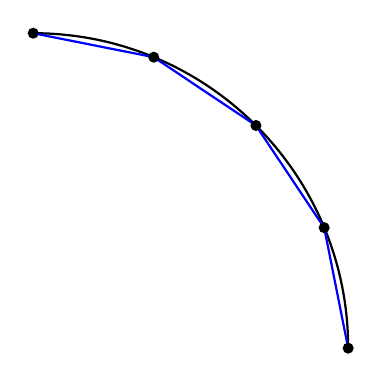
\begin{tikzpicture}
        \def\R{4}          % Radius of the arc
        \def\StartAng{0}   % Starting angle (0 is East)
        \def\EndAng{90}    % Ending angle (90 is North)
        \def\Segments{4}   % Number of chords
        \draw[thick] (\StartAng:\R) arc (\StartAng:\EndAng:\R);
        \pgfmathsetmacro{\step}{(\EndAng-\StartAng)/\Segments}

        \draw[blue, thick] (\StartAng:\R) 
            \foreach \i in {1,...,\Segments} {
                -- ({\StartAng + \i*\step}:\R)
            };
        \foreach \i in {0,...,\Segments} {
            \fill[black] ({\StartAng + \i*\step}:\R) circle (2pt);
        }
    \end{tikzpicture}
\end{center}

The procedure of decreasing the distance between the points to estimate the curve's length is essentially calculating the limit of the sum of the lengths of these (blue) straight lines as the distance between the points approaches zero. \uwave{In other words, the length of the curve is the limit of the sum of the lengths of the blue line segments.} 
\begin{center}
    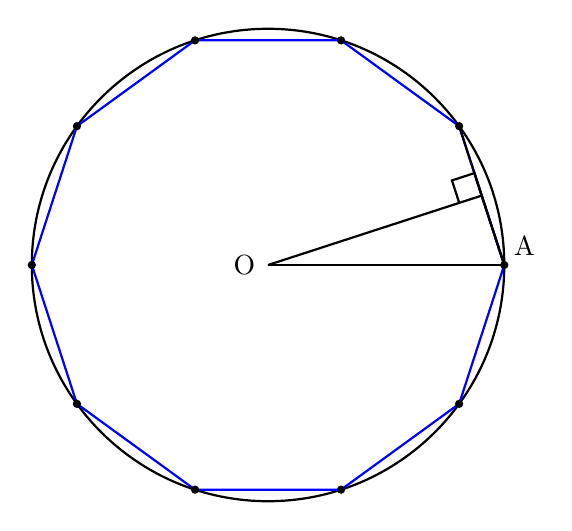
\begin{tikzpicture}
        \draw[thick] (0,0) circle (3cm);
        \draw[blue, thick] (0:3cm) 
            \foreach \angle in {36, 72, ..., 360}
            {
                -- (\angle:3cm)
            } -- cycle;
        \draw[thick, black] (0:3cm) -- (36:3cm);  
        \draw[black, thick] (0,0) -- (0:3cm);
        \node[above right] at (0:3cm) {A};  % label point A
        \draw[black, thick] (0,0) -- (18:{3*cos(18)});
        \draw[thick, black] (18:{3*cos(18)}) -- (0:3cm);
        \def\r{0.3}  % size of the right-angle mark
        \draw[black, thick] 
            (18:{3*cos(18)-\r}) -- ++(18+90:\r) -- ++(18:\r) -- ++(18-90:\r);
        \node at (-0.3,0) {O};              % center
        \foreach \angle in {0, 36, ..., 324}
        {
            \fill (\angle:3cm) circle (1.5pt);
        }
    \end{tikzpicture}
\end{center}

The perimeter of a regular $n$-gon inscribed in the unit circle is $2n\sin \frac{180^{\circ}}{n}$. Let the half perimeter be $L_{n} = n\sin\frac{180^{\circ}}{n}$. We then have a sequence $\left\{L_{n}\right\}$.

\begin{example}{}{exp_3_7_5}
    Prove that the sequence $\left\{L_{n}\right\}$ with $L_{n} = n\sin\frac{180^{\circ}}{n}$ converges.
\end{example}

\begin{proof}{MyExpColor}
    Let $t = \frac{180^{\circ}}{n(n+1)}$ and $n \geq 3$ is obvious, so $t\leq15^{\circ}, nt \leq 45^{\circ}$. Then
    \[
        \tan nt = \tan \left( \left( n-1\right)t + t\right) = \frac{\tan (n-1)t + \tan t}{1- \tan(n-1)t \cdot \tan t} \textcolor{red}{\,>\,} \tan (n-1)t + \tan t,
    \]
    In the red inequality, we can verify that $(n-1)t = \frac{(n-1)180^{\circ}}{n(n+1)}$, which decreases for $n \geq 3$ and takes value in $\left(0^{\circ}, 30^{\circ}\right]$ Then $\tan (n-1)t \cdot \tan t \leq \tan30^{\circ}\cdot\tan45^{\circ} < 1$. Thus we have
    \[
        \tan nt = \tan \left( \left( n-1\right)t + t\right) > \textcolor{blue}{\tan (n-1)t} + \tan t.
    \]
    For the blue term we have
    \[
        \tan (n-1)t = \tan \left( \left( n-2\right)t + t\right) > \tan(n-2)t + \tan t.
    \]
    Therefore we have 
    \[
        \tan(n-1)t + \tan t  > \tan (n-2)t + 2\tan t.
    \]
    The pattern should be obvious now, that is
    \[
        \tan nt > \tan(n-1)t + \tan t > \tan (n-2)t + 2\tan t > \dots > \tan (n-n)t + n\tan t = n \tan t.
    \]
    That is we have shown $\tan nt > n \tan t$. 

    Also,
    \begin{align*}
        \sin(n+1)t &= \sin nt \cos t + \cos nt \sin t \\
                &= \sin nt \cos t + \sin nt \cos t \frac{\tan t}{\tan nt} \\
                &= \sin nt \underbrace{\cos t}_{ \leq 1} \cdot \bigg( 1+ \underbrace{\frac{\tan t}{\tan nt}}_{< \frac{1}{n}}\bigg) \\
                &< \sin nt \cdot \left(\frac{n+1}{n}\right)
    \end{align*}
    That is $\sin(n+1)t < \sin nt \cdot \left(\frac{n+1}{n}\right)$. Substitute $t = \frac{180^{\circ}}{n(n+1)}$ to get
    \begin{align*}
        \sin \frac{180^{\circ}}{n} &< \sin \frac{180^{\circ}}{n+1} \cdot \left(\frac{n+1}{n}\right) \\
        n\sin \frac{180^{\circ}}{n} &< (n+1)\sin \frac{180^{\circ}}{n+1}
    \end{align*}
    We get
    \[
    L_{n} = n\sin \frac{180^{\circ}}{n} < (n+1)\sin \frac{180^{\circ}}{n+1} = L_{n+1}.
    \]
    Therefore, we have shown the sequence $\{L_{n}\}$ is monotonically increasing. For the boundedness, lets start with the area of a regular $n$-gon inscribed in the unit circle. Let this area be $S_{n}$, we know 
    \[
    S_{n} = 2n\cdot\frac{1}{2}\sin\frac{180^{\circ}}{n}\cdot\cos\frac{180^{\circ}}{n} < 4.
    \]
    That is 
    \[
        n\sin\frac{180^{\circ}}{n} < \frac{4}{\cos\frac{180^{\circ}}{n}} < 8.
    \]
    The LHS equals $L_{n}$ therefore we have $L_{n} < 8, \forall\, n \geq 3$. Thus the sequence $\left\{L_{n}\right\}$ is bounded. By the Monotone Convergence Theorem, the sequence $\left\{L_{n}\right\}$ is convergent.
    Therefore, we know that the limit of the sequence $\left\{L_{n}\right\}$ exist and is the half of the perimeter of the unit circle which is $\pi$. That is
    \[
        \lim\limits_{n\to\infty}L_{n} = \lim\limits_{n\to\infty}n\sin\frac{180^{\circ}}{n} = \pi.
    \]
\end{proof}

\begin{remark}
We can keep going to calculate the area of the unit circle. We have calculated the area of a regular $n$-gon inscribed in the unit circle, $S_{n}$. Now we want to calculated the are of a regular $n$-gon circumscribed about a unit circle, $S_{n}^{\prime}$.

\begin{center}
    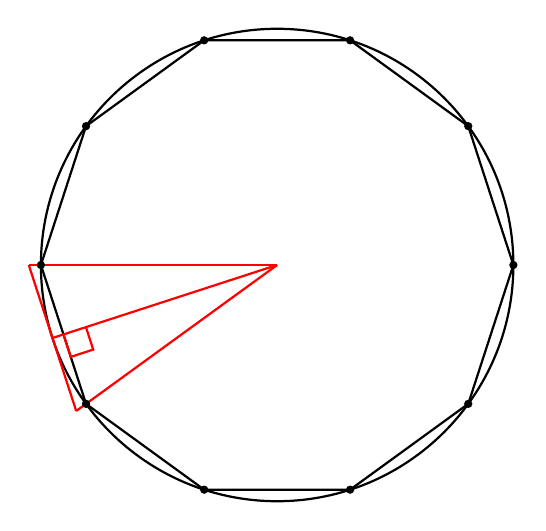
\begin{tikzpicture}
        \draw[thick] (0,0) circle (3cm);
        \draw[thick] (0:3cm)
            \foreach \angle in {36, 72, ..., 360}
            {
                -- (\angle:3cm)
            } -- cycle;
        \coordinate (A) at (180:{3/cos(18)});   % one endpoint (used for the triangle)
        \coordinate (B) at (216:{3/cos(18)});   % the other endpoint
        \coordinate (C) at (198:3cm);
        \draw[red, thick] (A) -- (B);
        \coordinate (O) at (0,0);
        \coordinate (M) at (198:{3*cos(18)});
        \draw[thick, red] (O) -- (A);
        \draw[thick, red] (O) -- (C);
        \draw[thick, red] (O) -- (B);
        \def\r{0.3}  % size of the mark
        \draw[red, thick]
            (198:{3*cos(18)-\r}) -- ++(198+90:\r) -- ++(198:\r) -- ++(198-90:\r);
        \foreach \angle in {0, 36, ..., 324}
        {
            \fill (\angle:3cm) circle (1.5pt);
        }
    \end{tikzpicture}
\end{center}

We have $S_{n}^{\prime} = n\tan\frac{180^{\circ}}{n} =  \frac{n\sin\frac{180^{\circ}}{n}}{\cos\frac{180^{\circ}}{n}}$. We also have this inequality for the area of the unit circle $S$:
\[
    n\sin\frac{180^{\circ}}{n}\cos\frac{180^{\circ}}{n}=S_{n} < S < S_{n}^{\prime} = n\tan\frac{180^{\circ}}{n} =  \frac{n\sin\frac{180^{\circ}}{n}}{\cos\frac{180^{\circ}}{n}}
\]
Since $n\sin\frac{180^{\circ}}{n} \xrightarrow{n\to\infty} \pi$ and $\cos\frac{180^{\circ}}{n} \xrightarrow{n\to\infty}1$, therefore when $n \to \infty$ we have 
\[
    \pi = \lim\limits_{n\to\infty}S_{n} < \lim\limits_{n\to\infty}S < \lim\limits_{n\to\infty}S_{n}^{\prime} = \pi
\]
By the squeeze theorem, we have $\lim\limits_{n\to\infty}S = \pi$, which verifies that the area of a unit circle is indeed $\pi$.
\end{remark}

\begin{remark}
    We have shown, in the example above, that if the perimeter of a circle is $2\pi$ by definition, then the area of the circle is $\pi$. 
\end{remark}

Now let's talk about $e$.
\begin{example}{}{exp_3_7_6}
    We have two sequences $x_{n} = \left(1+ \frac{1}{n}\right)^{n}$ and $y_{n} = \left(1+ \frac{1}{n}\right)^{n+1}$. Do the sequences $\{x_{n}\}$ and $\{y_{n}\}$ converge? If so, find their respective limits.
\end{example}
\begin{proof}{MyExpColor}
    For the sequence $x_{n}$ we have 
    \[
    x_{n} = \left(1+\frac{1}{n}\right)^{n} \cdot 1 \textcolor{red}{\,\leq\,} \Bigg(\frac{n\cdot\left(1+\frac{1}{n}\right) + 1}{n+1}\Bigg)^{n+1} = \Bigg(1 + \frac{1}{n+1}\Bigg)^{n+1} = x_{n+1}
    \]
    That is the sequence $\{x_{n}\}$ is increasing, therefore $\{x_{n}\}$ has upper limit. For $\{y_{n}\}$, we have 
    \[
    \frac{1}{y_{n}} = \left(\frac{n}{n+1}\right)^{n+1} \cdot 1 \leq \Bigg(\frac{(n+1)\cdot\left(\frac{n}{n+1}\right) + 1}{n+2}\Bigg)^{n+2} = \Bigg(\frac{n+1}{n+2}\Bigg)^{n+2} = \frac{1}{y_{n+1}}
    \]
    The sequence $\{y_{n}\}$ is decreasing, therefore $\{y_{n}\}$ has lower limit. It is obvious that 
    \[
    2 < x_{1} < x_{n} < y_{n} \leq y_{1} = 4.
    \]
    Therefore, we know $\lim\limits_{x\to\infty}x_{n}$ and $\lim\limits_{n\to\infty}y_{n}$ converge. Also,
    \[
    y_{n} = x_{n}\left(1 + \frac{1}{n}\right)
    \]
    Taking limit on both side, we get $\lim\limits_{x\to\infty}x_{n} = \lim\limits_{n\to\infty}y_{n}$. Using the binomial theorem, we have 
    \begin{align*}
        \lim\limits_{n\to\infty} x_{n} &= \lim\limits_{n\to\infty}\left(1+\frac{1}{n}\right)^{n} \\
        &= \lim\limits_{n\to\infty}\sum_{k=0}^{\infty} \binom{n}{k}\frac{1}{n^{k}} \\ 
        &= \lim\limits_{n\to\infty}\sum_{k=0}^{\infty} \frac{n\cdot(n-1) \dots (n-k+1)}{k!}\cdot\frac{1}{n^{k}} \\
        &= \lim\limits_{n\to\infty}\sum_{k=0}^{\infty} \frac{n\cdot(n-1) \dots (n-k+1)}{n^{k}}\cdot\frac{1}{k!} \\
        &= \lim\limits_{n\to\infty}\sum_{k=0}^{\infty} \textcolor{red}{\frac{(n-0)\cdot(n-1) \dots \left(n-(k-1)\right)}{n^{k}}}\cdot\frac{1}{k!} \\
        &= \lim\limits_{n\to\infty}\sum_{k=0}^{\infty} \textcolor{red}{\prod_{j=0}^{k-1}\frac{n-j}{n}}\cdot\frac{1}{k!} \\
        &= \lim\limits_{n\to\infty}\sum_{k=0}^{\infty} \textcolor{red}{\prod_{j=0}^{k-1}\left(1 - \frac{j}{n}\right)}\cdot\frac{1}{k!} \\
        &= \sum_{k=0}^{\infty}\frac{1}{k!} \\
        &= e
    \end{align*}
\end{proof}

\begin{note}
    The red inequality is due to the geometric mean being less than or equal to the arithmetic mean. There are $n+1$ terms multiplied together on the LHS of the red inequality.
\end{note}

\begin{example}{}{}
    Let $a_{n} = 1 + \frac{1}{2^{p}} + \frac{1}{3^{p}} + \dots + \frac{1}{n^{p}}$, with $p>0$. It is obvious that $\{a_{n}\}$ is increasing. Prove that when $p>1$ the sequence $\{a_{n}\}$ converges and when $p \leq 1$ it diverges to infinity.
\end{example}

\begin{proof}{MyExpColor}
    For $p > 1$, let $\frac{1}{2^{p-1}} = r$. It is obvious that $0 < r < 1$. Then we have
    \begin{align*}
        &\frac{1}{2^{p}} + \frac{1}{3^{p}} \leq \frac{2}{2^{p}} = r \\
        &\frac{1}{4^{p}} + \frac{1}{5^{p}} + \frac{1}{6^{p}} + \frac{1}{7^{p}} \leq \frac{4}{4^{p}} = r^{2} \\
        & \frac{1}{8^{p}} + \frac{1}{9^{p}} + \dots + \frac{1}{15^{p}} \leq \frac{8}{8^{p}} = r^{3} \\
        & \vdots \\
        & \frac{1}{(2^{k})^{p}} + \frac{1}{(2^{k} + 1)^{p}} + \dots + \frac{1}{(2^{k+1}-1)^{p}} \leq \frac{2^{k}}{(2^{k})^{p}} = \frac{1}{(2^{k})^{p-1}} = r^{k}
    \end{align*}
    It should now be obvious that $\forall\, n$, $a_{n} < a_{2^{n}-1} < 1 + r^{2} + \dots + r^{n-1} = \frac{1}{1-r}$. Therefore, the sequence $\{a_{n}\}$ is bounded above so as to have an upper limit. That is $\lim\limits_{n\to\infty}a_{n}$ exists. \\
    For $0 < p \leq 1$, we have 
    \begin{align*}
        &\frac{1}{2^{p}} \geq \frac{1}{2} \\
        &\frac{1}{3^{p}} + \frac{1}{4^{p}} \geq \frac{1}{4^{p}} + \frac{1}{4^{p}} > \frac{1}{4} + \frac{1}{4} = \frac{1}{2} \\
        &\frac{1}{5^{p}} + \frac{1}{6^{p}} + \frac{1}{7^{p}} + \frac{1}{8^{p}} \geq \frac{1}{8^{p}} + \frac{1}{8^{p}} + \frac{1}{8^{p}} + \frac{1}{8^{p}} > \frac{1}{8} + \frac{1}{8} + \frac{1}{8} + \frac{1}{8} = \frac{1}{2} \\
        &\vdots \\
        &\frac{1}{(2^{k} + 1)^{p}} + \frac{1}{(2^{k} + 2)^{p}} + \dots + \frac{1}{(2^{k+1})^{p}} \geq \frac{2^{k}}{(2^{k+1})^{p}} > \frac{2^{k}}{2^{k+1}} = \frac{1}{2}
    \end{align*}
    It should now be obvious that as $n \to \infty$, the sequence $\{a_{n}\}$ is not bounded above.
\end{proof}

\begin{note}
    Be aware that 
    \begin{align*}
        a_{n} &= 1 + \frac{1}{2} + \frac{1}{3} + \dots + \frac{1}{n} \\
        \sum_{n=1}^{\infty}\frac{1}{n} &= 1 + \frac{1}{2} + \frac{1}{3} + \dots + \frac{1}{n} + \dots
    \end{align*}
    are different.
\end{note}

Let us compare two quantities, $1 + \frac{1}{2} + \frac{1}{3} + \dots + \frac{1}{n}$ and $\ln n$, which both tend to positive infinity, by subtracting one from the other. 

\begin{example}{}{}
    Let $b_{n} = 1 + \frac{1}{2} + \frac{1}{3} + \dots + \frac{1}{n} - \ln n$ and show that the sequence $\{b_{n}\}$ converges.
\end{example}
\begin{proof}{MyExpColor}
    Recall that we have $\left(1+\frac{1}{n}\right)^{n} < e < \left(1+\frac{1}{n}\right)^{n+1}$. From the right inequality, we get 
    \[
    1 < (n+1)\ln \frac{n+1}{n} \implies \frac{1}{n+1} < \ln \frac{n+1}{n}.
    \]
    From the left inequality, we get
    \[
        n \ln\frac{n+1}{n} < 1 \implies \ln\frac{n+1}{n} < \frac{1}{n}.
    \]
    That is 
    \[
    \frac{1}{n+1} \textcolor{red}{<} \ln \frac{n+1}{n} \textcolor{blue}{<} \frac{1}{n}.
    \]
    Next we will verify if $\{b_{n}\}$ converges or not.
    \[
        b_{n+1} - b_{n} = \frac{1}{n+1} - \ln (n+1) + \ln n = \frac{1}{n+1} - \ln\frac{n+1}{n} 
    \]
    Using the red inequality, we know that $b_{n+1} - b_{n} < 0$. That is 
 the sequence $\{b_{n}\}$ is strictly decreasing. We also have
     \begin{align*}
         b_{n} &= 1 + \frac{1}{2} + \frac{1}{3} + \dots + \frac{1}{n} - \ln n \\
         &> \ln \frac{2}{1} + \ln\frac{3}{2} + \ln\frac{4}{3} + \dots + \ln\frac{n+1}{n} -\ln n \\
         &= \ln (n+1) - \ln n = \ln\frac{n+1}{n} > 0
     \end{align*}
     Therefore, we conclude that the sequence $\{b_{n}\}$ converges.    
\end{proof}

\begin{note}
    We briefly touch the limit of the sequence $\{b_{n}\}$ here, which is called the \textbf{Euler Constant} or \textbf{Euler-Mascheroni constant} and it is denoted $\gamma = \lim\limits_{n\to\infty} \sum\limits_{k=1}^{n} \frac{1}{k} - \ln n \simeq 0.5772156649....$, an irrational number.
\end{note}
\begin{remark}
    As we can see that the difference between these two infinite quantities, the sequence $\{a_{n}\}$ and $\ln n$, are not too big as $n$ goes to infinity. In other words, the difference between these two infinite quantities is the \textbf{Euler Constant}, $\gamma$, as $n$ approaches infinity. \uwave{We conclude that the two infinite quantities are \textbf{asymptotically equivalent} or \textbf{equivalent}.} 
\end{remark}

\begin{example}{}{}
    Prove $\lim\limits_{n\to\infty}\left(\frac{1}{n+1} + \frac{1}{n+2} + \frac{1}{n+3} + \dots + \frac{1}{2n}\right) = \ln 2$.
\end{example}

\begin{proof}{MyExpColor}
    Recall in the last example $b_{n} = 1 + \frac{1}{2} + \frac{1}{3} + \dots + \frac{1}{n} - \ln n$ and $b_{n} \xrightarrow{n \to \infty}{\gamma}$. It should be obvious that $b_{2n} \xrightarrow{n \to \infty}{\gamma}$. The limit of $\{b_{n}\}$ is $\gamma$, so no matter how large $n$ is the limit of the sequence $\{b_{n}\}$, $\{b_{2n}\}$, or $\{b_{5n}\}$ will always be $\gamma$.
    \begin{align*}
        b_{n} &= 1 + \frac{1}{2} + \frac{1}{3} + \dots + \frac{1}{n} - \ln n \\ 
        b_{2n} &= 1 + \frac{1}{2} + \frac{1}{3} + \dots + \frac{1}{2n} - \ln 2n \\
        b_{2n} - b_{n} &= \frac{1}{n+1} + \frac{1}{n+2} + \frac{1}{n+3} + \dots + \frac{1}{2n} - \ln 2n + \ln n \\
        &= \frac{1}{n+1} + \frac{1}{n+2} + \frac{1}{n+3} + \dots + \frac{1}{2n} - \ln2 \,\xrightarrow{n \to\infty}{0}
    \end{align*}
    It is obvious that we take the limit we have what we want to show.
\end{proof}

\begin{note}
    Before proving, it is worth to point out that 
    \[
        \lim\limits_{n\to\infty}\left(\frac{1}{n+1} + \frac{1}{n+2} + \frac{1}{n+3} + \dots + \frac{1}{2n}\right) \textcolor{red}{\neq} \lim\limits_{n\to\infty}\frac{1}{n+1} + \lim\limits_{n\to\infty}\frac{1}{n+2} + \lim\limits_{n\to\infty}\frac{1}{n+3} + \dots + \lim\limits_{n\to\infty}\frac{1}{2n}
    \]
    We have discussed this reason why it is not the case in previous lectures. In short, the number of terms inside the limit increases as $n$ goes to infinity.
\end{note}


\begin{example}{}{}
    Find out if the sequence $d_{n} = 1 - \frac{1}{2} + \frac{1}{3} - \frac{1}{4} + \dots + (-1)^{n+1}\frac{1}{n}$ converges.
\end{example}

\begin{proof}{MyExpColor}
    Recall, 
    \begin{align*}
        b_{n} &= 1 + \frac{1}{2} + \frac{1}{3} + \dots + \frac{1}{n} - \ln n \\
        b_{2n} &= 1 + \frac{1}{2} + \frac{1}{3} + \dots + \frac{1}{2n} - \ln 2n \\ 
        b_{2n} - b_{n} &= 1 + (\frac{1}{2} - 1) + \frac{1}{3} + (\frac{1}{4} - \frac{1}{2}) + \dots + (\frac{1}{2n} - \frac{1}{n}) -\ln 2n + \ln n \\
        &= 1 - \frac{1}{2} + \frac{1}{3} - \frac{1}{4} + \dots -\frac{1}{2n} - \ln 2 \\
        &= d_{n} - \ln 2 \,\xrightarrow{n \to \infty}{0}
    \end{align*}
    Thus, we have $d_{n} \xrightarrow{n\to\infty}{\ln 2}$.
\end{proof}

It is a good time to have a summary of the previous several examples and to summarize it yourself and try to learn the techniques used in proving these problems.

Before talking about a very important theorem, \textbf{The Nested Intervals Theorem}, let us introduce a definition.



\subsection{The Nested Intervals Theorem}
\begin{definition}{Nested Closed Intervals}{def_3_7_1}
    If a sequence of closed intervals $I_{n} = \{[a_{n}, b_{n}]\}$ satisfy:

    \begin{enumerate}[topsep=10pt, itemsep=5pt]
        \item $[a_{n}, b_{n}] \supseteq [a_{n+1}, b_{n+1}]$ for $n = 1, 2, 3, \dots$; and
        \item $b_{n} - a_{n} \,\xrightarrow{n \to\infty}{0}$, then 
    \end{enumerate}
    then the sequence of intervals $I_{n}$ is called the Nested Closed Intervals.
\end{definition}

\begin{theorem}{The Nested Intervals Theorem}{}
    For a nested closed intervals $\{[a_{n}, b_{n}]\}$, there exists an unique real number $\xi$ such that $\xi \in [a_{n}, b_{n}], \forall\, n \in \mathbb{N}$ and $\lim\limits_{n\to\infty}a_{n} = \lim\limits_{n\to\infty}b_{n} = \xi$.
\end{theorem}

\begin{proof}{MyThmColor}
    By the definition of nested closed intervals, it is obvious that 
    \[
        a_{1}\leq \dots \leq a_{n-1} \leq a_{n} < b_{n} \leq b_{n-1} \leq \dots \leq b_{1}.
    \]
    Hint: as $n$ increases the closed intervals are nested or the intervals are shrinking. 
    
    It should also be obvious that the sequence $\{a_{n}\}$ is monotonically increasing with an upper bound $b_{1}$, and the sequence $\{b_{n}\}$ is monotonically decreasing with a lower bound $a_{1}$. Therefore $\{a_{n}\}$ and $\{b_{n}\}$ converge. Naturally, we can assume $\lim\limits_{n\to\infty}a_{n} = \xi \in \mathbb{R}$, or $\xi$ is the supremum of $\{a_{n}\}$, then $\lim\limits_{n\to\infty}b_{n} = \lim\limits_{n\to\infty}\left(a_{n} + (b_{n} - a_{n})\right) = \lim\limits_{n\to\infty}a_{n} + \lim\limits_{n\to\infty}(b_{n}-a_{n}) = \xi - 0 = \xi$. That is $\lim\limits_{n\to\infty}b_{n} = \xi$ as well. Also, we know $\xi$ is the infimum of $\{b_{n}\}$, that is $a_{n} \leq \xi \leq b_{n}$; equivalently, $\xi \in [a_{n}, b_{n}], \forall\, n\in \mathbb{N}$. We only need to show the uniqueness of $\xi$. 

    To show the uniqueness of $\xi$, we assume $\exists\, \xi^{\prime} \in [a_{n}, b_{n}], \forall\, n \in \mathbb{N}$ such that $a_{n} \leq \xi^{\prime} \leq b_{n}$, then we take the limit of the inequalities and apply the squeeze theorem to get $\xi \leq \xi^{\prime}\leq \xi$. It is straightforward that $\xi^{\prime} = \xi$.
\end{proof}

\begin{theorem}{}{thm_3_7_3}
    The real number set, $\mathbb{R}$, is uncountable.
\end{theorem}

\begin{proof}{MyThmColor}
We use prove by contradiction and apply the Nested Intervals Theorem to prove this theorem. 

   Suppose $\mathbb{R}$ is countable, for the sake of contradiction, that is we can list the set of real numbers as $\mathbb{R} = \{x_{1}, x_{2}, x_{3}, \dots, x_{n}, \dots\}, \forall\, n \in \mathbb{N}$. Then to show this is not the case, we only need to find one real number that is not listed. To do so, we first construct a closed interval $[a_{1}, b_{1}]$ such that $x_{1} \notin [a_{1}, b_{1}]$, then we construct a new closed interval by dividing $[a_{1}, b_{1}]$ into three parts, $\left[a_{1}, \frac{2a_{1}+b_{1}}{3}\right], \left[\frac{2a_{1}+b_{1}}{3}, \frac{a_{1}+2b_{1}}{3}\right], \left[\frac{2a_{1}+b_{1}}{3}, b_{1}\right]$. It is obvious that $x_{2}$ will be in only one of the three. So, pick any interval from the three that does not contain $x_{2}$ and name it $[a_{2}, b_{2}]$. In other words, we have $x_{2} \notin [a_{2}, b_{2}]$, and more importantly, $[a_{1}, b_{1}] \supseteq [a_{2}, b_{2}]$. Next, we divide $[a_{2}, b_{2}]$ into three parts and name it $[a_{3}, b_{3}]$ which does not have $x_{3}$ in it, that is $x_{3} \notin [a_{3}, b_{3}]$ and $[a_{1}, b_{1}] \supseteq [a_{2}, b_{2}] \supseteq [a_{3}, b_{3}]$. We apply this method and every time we construct a new interval $[a_{n}, b_{n}]$, we know that 
   \begin{enumerate}
       \item[1.] $[a_{n-1}, b_{n-1}] \supseteq [a_{n}, b_{n}]$
       \item[2.] $b_{n}-a_{n} \xrightarrow{n\to\infty}{0}$. This is because the way we create these new intervals.
       \item[3.] $x_{n} \notin [a_{n}, b_{n}]$.
   \end{enumerate}
   By the Nested Intervals Theorem, we know that there exists a unique real number $\xi \in [a_{n}, b_{n}]$ and we know $\xi \neq x_{n}$. This shows that $\xi$ is not listed in $\mathbb{R} = \{x_{1}, x_{2}, x_{3}, \dots, x_{n}, \dots\}, \forall\, n \in \mathbb{N}$. Thus, $\mathbb{R}$ is uncountable.
\end{proof}
\begin{note}
    It is not possible that $x_{2} \notin [a_{2}, b_{2}]$ but $x_{1} \in [a_{2}, b_{2}]$, since the new interval, $[a_{2}, b_{2}]$, is smaller than the previous one, $[a_{1}, b_{1}]$, which does not have $x_{1}$. 
\end{note}



\subsection{Subsequence}
We give a definition of the subsequence.
\begin{definition}{}{def_3_7_2}
    Given a sequence $\{x_{n}\}$ and a list of strictly increasing integers
    \[
        n_{1} < n_{2} < n_{3} < \dots < n_{k} < \dots, \forall\, k \in \mathbb{N},
    \]
    then we say $x_{n_{1}}, x_{n_{2}}, x_{n_{3}}, \dots, x_{n_{k}}, \dots$ is a \textbf{subsequence} of the sequence $\{x_{n}\}$ and denoted as $\{x_{n_{k}}\}, \forall\, k \in \mathbb{N}$.
\end{definition}

\begin{note}
    We observe that $k$ indicates that $x_{n_{k}}$ is the $k$-th term in the subsequence and $n_{k}$ shows that $x_{n_{k}}$ is the $n_{k}$-th term in the original sequence. Then it is obvious to have two properties:
    
    \begin{enumerate}[topsep=10pt, itemsep=5pt]
        \item $n_{k} \geq k, \forall\, k\in\mathbb{N}$,
        \item $n_{j} > n_{k}, \forall\, j > k$.
    \end{enumerate}
\end{note}

\begin{theorem}{}{}
    If a sequence $\{x_{n}\}$ converges to $a$ then any of its subsequence $\{x_{n_{k}}\}$ converges to $a$. 
\end{theorem}

\begin{proof}{MyThmColor}
    Let $\lim\limits_{n\to\infty}x_{n} = a$. We want to show $\lim\limits_{k\to\infty}x_{n_{k}} = a$ as well. That is equivalent to show that there $\forall\, \epsilon > 0$ we can find a $K$ such that $\forall\, k > K$ there is $\vert x_{n_{k}} - a \vert < \epsilon$. \\
    Rewriting $\lim\limits_{n\to\infty}x_{n} = a$, we have $\forall\, \epsilon > 0$ we can find an $N$ such that $\forall\, n > N$ there is $\vert x_{n} - a \vert < \epsilon$. 
    \uwave{By letting $K = N$}, \uwave{we can always find $k > K = N$} and using the property of subsequence we know that we have $n_{k} \geq N$. So, we know that \uwave{$\forall\, \epsilon > 0$}, \uwave{we can find an $N = K$} such that \uwave{$\forall\, n_{k} \geq k > K=N$} there is \uwave{$\vert x_{n_{k}} - a \vert < \epsilon$}.
\end{proof}

\begin{remark}
    This theorem is powerful in proving some sequence diverges. As long as we can find two subsequences (of a sequence) converges to different limit then we know the sequence does not converge.
\end{remark}

\begin{corollary}{}{}
    If a sequence $\{x_{n}\}$ has two subsequences that converge to two different limits, then the sequence $\{x_{n}\}$ diverges.
\end{corollary}

\begin{example}{}{}
    Show that the sequence $\{\sin \frac{n\pi}{4}\}$ diverges.
\end{example}
\begin{proof}{MyExpColor}
    Let the first sequence of integers be $n_{k}^{(1)} = 4k$ and another sequence of integers be $n_{k}^{(2)} = 8k + 2$. Then it should be obvious that $\{x_{n_{k}^{(1)}}\}$ has a limit $0$, while $\{x_{n_{k}^{(2)}}\}$ has a limit $1$. So, $\{\sin \frac{n\pi}{4}\}$ diverges.
\end{proof}



\subsection{Bolzano-Weierstrass Theorem}
\begin{theorem}{\quad Bolzano-Weierstrass Theorem}{thm_3_7_6}
    Every bounded sequence has a convergent subsequence.
\end{theorem}

\begin{proof}{MyThmColor}
    Given a sequence $\{x_{n}\}$ is bounded that is $a_{1} \leq x_{n} \leq b_{1} \Leftrightarrow x_{n} \in [a_{1}, b_{1}], \forall\, n \in \mathbb{N}$. Now, we divide $[a_{1}, b_{1}]$ into two intervals, $[a_{1}, \frac{a_{1} + b_{1}}{2}]$ and $[\frac{a_{1} + b_{1}}{2}, b_{1}]$. In the two intervals, there must be at least one contains infinitely many terms of $\{x_{n}\}$ and we call it $[a_{2}, b_{2}]$.
    Now we divide $[a_{2}, b_{2}]$ into two smaller interval, $[a_{2}, \frac{a_{2}+b_{2}}{2}]$ and $[\frac{a_{2}+b_{2}}{2}, b_{2}]$. It is obvious that at least one of the two intervals contains infinitely many terms in $\{x_{n}\}$. We keep doing this by spiting the interval into two intervals and choose the one that contains infinitely many terms from $\{x_{n}\}$ to be $[a_{n}, b_{n}]$. Thus, we have a Nested Closed Intervals $\{[a_{n}, b_{n}]\}$, there exists a real number $\xi$ such that $\xi \in [a_{n}, b_{n}]$ and $\lim\limits_{n\to\infty}a_{n} = \lim\limits_{n\to\infty}b_{n} = \xi$. Now we construct a subsequence and show its limit is $\xi$. In $[a_{1}, b_{1}]$, we can find $x_{n_{1}}$. In $[a_{2}, b_{2}]$, we can find $x_{n_{2}}$, with $n_{2} > n_{1}$. (Why we can always find $n_{2} > n_{1}$? Since the interval contains infinitely many terms from $\{x_{n}\}$) .In $[a_{3}, b_{3}]$, we can find $x_{n_{3}}$, with $n_{3} > n_{2}$. The pattern follows, thus in $[a_{k}, b_{k}]$, we can find $x_{n_{k}}$, with $n_{k} > n_{k-1}$. Thus, we constructed a subsequence $\{x_{n_{k}}\}$ from the original sequence $\{x_{n}\}$. It should be obvious that $a_{k} \leq x_{n_{k}} \leq b_{k}$ and since $\lim\limits_{k\to\infty}a_{k} = \xi = \lim\limits_{k\to\infty}b_{k}$, then by the squeeze theorem, we arrive at $\lim\limits_{k\to\infty}x_{n_{k}} = \xi$.
\end{proof}

\begin{note}
    An unbounded sequence is not necessarily an infinite quantity. For example the sequence 
    \[
        \{2, 3, 2, 4, 2, 5, 2, 6, \dots \}
    \]
    is increasing but the odd number of terms in this sequence stay at $2$. This contradicts with the definition of the infinite quantity as $n$ goes to infinity.
\end{note}

\begin{theorem}{}{}
    An unbounded sequence has a subsequence that diverges to infinite.
\end{theorem}
\begin{proof}{MyThmColor}
    Let $\{x_{n}\}$ be an unbounded sequence, thus we can say $\forall\, M > 0$ we can always find infinitely many terms in $\{x_{n}\}$ such that
    \[
        \vert x_{n} \vert > M. 
    \]
    (Think about this. If we could only find finitely many terms in $\{x_{n}\}$ that is greater than $M$, then $\{x_{n}\}$ must be bounded.) 
    Let 
    \begin{align*}
        M_{1} &= 1, \exists\, \vert x_{n_{1}}\vert > 1; \\
        M_{2} &= 2, \exists\, \vert x_{n_{2}}\vert > 2; n_{2} > n_{1} \\
        M_{3} &= 3, \exists\, \vert x_{n_{3}}\vert > 3; n_{3} > n_{2}\\
        \dots \\
        M_{k} &= k, \exists\, \vert x_{n_{k}}\vert > k; n_{k} > n_{k-1}
    \end{align*}
    Note, we can always find $n_{k} > n_{k-1}$ since there are infinitely many terms in $\{x_{n}\}$ such that $\vert x_{n_{k}}\vert > M_{k}$. Then, we have constructed a subsequence $\{x_{n_{k}}\}$, with $\vert x_{n_{k}}\vert > k $. Therefore, $x_{n_{k}}$ diverges to infinity.
\end{proof}



\subsection{Cauchy Convergence Theorem}
We have studied \textbf{Monotone Convergence Theorem for Sequences} and this is a sufficiency theorem. In other words, the Monotone Convergence Theorem provides a sufficient condition for the convergence of a sequence, namely that it is monotone and bounded. That means if a sequence is bounded and not monotone then it may converge or diverge. 

The \textbf{Cauchy Convergence Theorem} is sufficient and necessary condition for the convergence of a sequence.

\begin{definition}{The Cauchy Sequence / Fundamental Sequence}{}  
    If a sequence $\{x_{n}\}$ satisfies: $\forall\, \epsilon > 0$, $\exists\, N $ such that $\forall\, m,n > N$ we have $\vert x_{n} -  x_{m}\vert < \epsilon$, then the sequence $\{x_{n}\}$ is called the \textbf{Cauchy Sequence}.
\end{definition}

\begin{note}
    In the definition above, we can safely change the condition $\forall\, m,n > N$ to $\forall\, m > n > N$, without altering anything. In other words, we just assume $m > n$.
\end{note}

\begin{example}{}{}
    Tell if $x_{n} = 1 + \frac{1}{2^{2}} + \frac{1}{3^{2}} + \dots + \frac{1}{n^{2}}$ is a Cauchy sequence?
\end{example}

\begin{proof}{MyExpColor}
    We have 
    \begin{align*}
        \vert x_{m} - x_{n}\vert &= 1 + \frac{1}{2^{2}} + \frac{1}{3^{2}} + \dots + \frac{1}{m^{2}} - \left( 1 + \frac{1}{2^{2}} + \frac{1}{3^{2}} + \dots + \frac{1}{n^{2}}\right) \\
        &= \frac{1}{(n+1)^{2}} + \frac{1}{(n+2)^{2}} + \dots + \frac{1}{m^{2}} < \frac{1}{n(n+1)} + \frac{1}{(n+1)(n+2)} + \dots + \frac{1}{(m-1)m} \\
        &= \left(\frac{1}{n} - \frac{1}{n+1}\right) + \left(\frac{1}{n+1} - \frac{1}{n+2}\right) + \dots + \left(\frac{1}{m-1} - \frac{1}{m}\right) \\ 
        &= \frac{1}{n} - \frac{1}{m} < \frac{1}{n}.
    \end{align*}
    \uwave{Let $N = \left\lfloor\frac{1}{\epsilon}\right\rfloor$}, we can show that \uwave{$\forall\, \epsilon > 0$}, we \uwave{can find an $N$} such that \uwave{$\forall\, m > n > N$}, we have \uwave{$\vert x_{m} - x_{n}\vert < \epsilon$}. Therefore, $\{x_{n}\}$ is a Cauchy sequence.
\end{proof}

\begin{example}{}{}
     Tell if $x_{n} = 1 + \frac{1}{2} + \frac{1}{3} + \dots + \frac{1}{n}$ is a Cauchy sequence?
\end{example}

\begin{proof}{MyExpColor}
    We have 
    \begin{align*}
        \vert x_{m} - x_{n}\vert &= \frac{1}{n+1} + \frac{1}{n+2} + \dots + \frac{1}{m}
    \end{align*}
    Let $m = 2n$, then we get
    \begin{align*}
        \vert x_{2n} - x_{n}\vert &= \frac{1}{n+1} + \frac{1}{n+2} + \dots + \frac{1}{2n} > n \cdot \frac{1}{2n} = \frac{1}{2}.
    \end{align*}
    Choose $\epsilon = \frac{1}{2}$, $\forall\, N, \exists\, m = 2n > n > N$ such that $\vert x_{2n} - x_{n}\vert > \frac{1}{2}$. In other words, the dynamic in the $\epsilon$-$N$ game is lost ($n$ is canceled when calculating the difference between $x_{m}$ and $x_{n}$), so no matter how large the $N$ we choose the difference between $x_{m}$ and $x_{n}$ will not be less than $\frac{1}{2}$, as long as $m = 2n$. Therefore, $x_{n}$ is not a Cauchy sequence.
\end{proof}

\begin{theorem}{Cauchy Convergence Theorem / The Completeness Theorem of the Real Numbers}{}
    The sufficient and necessary condition for a sequence, $\{x_{n}\}$, to converge is that it is a Cauchy sequence.
\end{theorem}

\begin{proof}{MyThmColor}
    (Cauchy sequence $\Leftarrow$ convergent sequence) 
    
    Assume $\lim\limits_{n\to\infty}x_{n} = a$, that is $\forall\, \epsilon >0$, we can find an $N$ such that $\forall\, n > N$, we have $\vert x_{n} - a\vert < \frac{\epsilon}{2}$. For the same $\epsilon$ and $N$, $\forall\, m > N$, we have $\vert x_{m} - a\vert < \frac{\epsilon}{2}$. Therefore, we know \uwave{$\forall\, \epsilon > 0$}, we can \uwave{find an $N$}, such that \uwave{$\forall\, m,n >N$}, we have \uwave{$\vert x_{m} - x_{n} \vert = \vert (x_{m} - a) - (x_{n} -a)\vert \leq \vert x_{m} - a\vert + \vert x_{n} - a\vert < \frac{\epsilon}{2} + \frac{\epsilon}{2} = \epsilon$}.
    
    (Cauchy sequence $\Rightarrow$ convergent sequence) 
    Briefly, we need to show that a Cauchy sequence is bounded then use Bolzano-Weierstrass Theorem to show that a bounded sequence has a convergent subsequence. Then show that the Cauchy sequence converge to that limit, so it is a convergent sequence. 

    Since $\{x_{n}\}$ is a Cauchy sequence, that is $\forall\, \epsilon > 0$ we can find an $N_{0}$ such that $\forall\, m, n > N_{0}$, we have $\vert x_{n} - x_{m}\vert < \epsilon \Leftrightarrow \vert x_{n}\vert < \vert x_{m} + \epsilon\vert$. Here we only need $m > N_{0}$ so we let $m = N_{0}+1$. Then we have $\vert x_{n}\vert < \vert x_{N_{0}+1} + \epsilon\vert$. Let $M = \max\left\{\vert x_{1}\vert, \vert x_{2}\vert, \dots, \vert x_{N_{0}+1}\vert, \vert x_{N_{0}+1} + \epsilon \vert  \right\}$, we have $\vert x_{n}\vert \leq M$. So $\{x_{n}\}$ is bounded. By Bolzano-Weierstrass Theorem, we know that there is a convergent subsequence $\{x_{n_{k}}\}$ and we let $\lim\limits_{k\to\infty} x_{n_{k}} = \xi$. (Now, we only need to show that $\{x_{n}\}$ indeed convergent to $\xi$).

    Again, by the definition of Cauchy sequence, we have \uwave{$\forall\, \epsilon > 0$}, we can \uwave{find an $N$} such that \uwave{$\forall\, m, n > N$} we have $\vert x_{n} - x_{m} \vert < \frac{\epsilon}{2}$. We can replace $m$ with $n_{k}$ as long as $k$ is large enough to make $n_{k} > N$. That is for very large $k$ so that $n_{k} > N$ (just like $m > N$), we have
    \[
        \vert x_{n} - x_{n_{k}}\vert < \frac{\epsilon}{2}
    \]
    then
    \begin{align*}
        \lim\limits_{k\to\infty}\vert x_{n} - x_{n_{k}}\vert &< \frac{\epsilon}{2} \\
        \vert x_{n} - \xi\vert &\leq \frac{\epsilon}{2} < \epsilon.
    \end{align*}
    Therefore, $\lim\limits_{n\to\infty}x_{n} = \xi$. This is $\{x_{n}\}$ is convergent.
\end{proof}

\noindent \textbf{The Geometric Contraction Condition} 

The Geometric Contraction Condition of a sequence $\{x_{n}\}$ is that it satisfies
\[
    \vert x_{n+1} - x_{n}\vert \leq k\vert x_{n} - x_{n-1}\vert, \quad 0<k<1.
\]
\begin{note}
    It is called \textbf{Geometric} Contraction Condition because 
\[
    \vert x_{n+1} - x_{n}\vert \leq k\vert x_{n} - x_{n-1}\vert \leq k^{2}\vert x_{n-1} - x_{n-2}\vert \leq \dots \leq k^{n}\vert x_{1} - x_{0}\vert, \quad0<k<1.
\]
\end{note}

If a sequence satisfies the Geometric Contraction Condition, then it converges.

\begin{example}{}{}
    Prove that if a sequence $\{x_{n}\}$ satisfies the Geometric Contraction Condition, then it converges.
\end{example}
\begin{proof}{MyExpColor}
    We just need to show a sequence satisfies the Geometric Contraction Condition is a Cauchy Sequence. 

    W.O.L.G., let us assume $m > n$. We have
    \begin{align*}
        \vert x_{m} - x_{n}\vert &= \vert (x_{m} - x_{m-1}) + (x_{m-1} - x_{m-2}) + \dots + (x_{n+1} - x_{n})\vert \\
        &\leq \vert (x_{m} - x_{m-1}) \vert + \vert (x_{m-1} - x_{m-2})\vert + \dots + \vert(x_{n+1} - x_{n})\vert \\
        &< k^{m-1}\vert x_{1} - x_{0}\vert + k^{m-2}\vert x_{1} - x_{0}\vert + \dots + k^{n}\vert x_{1} - x_{0}\vert \\
        &= k^{n}\vert x_{1} - x_{0}\vert \left( k^{m-1-n} + k^{m-2-n} + \dots + k + 1\right) \\
        &= k^{n}\vert x_{1} - x_{0}\vert \frac{1}{1-k} \,\xrightarrow{n\to\infty}{0}
    \end{align*}
    Thus, $\forall\, \epsilon > 0$, we have an $N$ such that $\forall\, m > n > N$ we have $\vert x_{m} - x_{n}\vert < \epsilon$. Therefore, the sequence $\{x_{n}\}$ satisfying the Geometric Contraction Condition is a Cauchy sequence. (So, it is convergent.)
\end{proof}



\subsection{Summary}
We need a summary! 
\begin{align*}
    1. \quad &\text{The Supremum Existence Theorem / (The Continuity Theorem of the Real Numbers)} \\
    &\quad \quad \quad \quad \quad \quad \quad \Downarrow \\
    2. \quad &\text{The Monotone (Bounded Sequence) Convergence Theorem} \\
    &\quad \quad \quad \quad \quad \quad \quad \Downarrow \\
    3. \quad &\text{The Nested Closed Interval Theorem}\\
    &\quad \quad \quad \quad \quad \quad \quad \Downarrow \\
    4. \quad &\text{The Bolzano-Weierstrass Theorem} \\
    &\quad \quad \quad \quad \quad \quad \quad \Downarrow \\
    5. \quad &\text{The Cauchy Convergence Theorem / (The Completeness Theorem of the Real Numbers) }
\end{align*}
\begin{note}
    The set of rational numbers is not complete. A quick example: the set $\left\{\left(1+\frac{1}{n}\right)^{n}\right\}$ is a set of rational numbers, but $\lim\limits_{n\to\infty}\left(1 + \frac{1}{n}\right)^{n} = e$, which is an irrational number.
\end{note}

Surprisingly or not so surprise, these five theorems above are equivalent, meaning assuming any one of these theorems as true, we can prove the other four. 

We will show their equivalence by using The Cauchy Convergence Theorem to prove The Nested Closed Interval Theorem and then to The Supremum Existence Theorem.

\begin{example}{}{}
    Using the Cauchy Convergence Theorem, we can prove the Nested Closed Interval Theorem.
\end{example}
\begin{proof}{MyExpColor}
    To prove the Nested Closed Intervals Theorem, we at least need to have a nested closed intervals. Given a nested closed interval $\{[a_{n}, b_{n}]\}$. That is it has two properties: $[a_{n+1}, b_{n+1}] \subseteq [a_{n}, b_{n}]$ and $b_{n}-a_{n} \xrightarrow{n\to\infty}{0}$. We need to show that there is a unique limit $\xi \in [a_{n}, b_{n}]$.

    Assuming $m > n$, by the definition of a nested closed interval, it is obvious that $[a_{m}, b_{m}] \subseteq [a_{n}, b_{n}]$. Equivalently we have 
    \[
        a_{m} - a_{n} < b_{n} - a_{n} \xrightarrow{n\to\infty}{0} 
    \]
    We proved the sequence $\{a_{n}\}$ is a Cauchy sequence. W.O.L.G., assuming $\lim\limits_{n\to\infty}a_{n} = \xi$, then we know $\lim\limits_{n\to\infty}b_{n} = \xi$. Since $\{a_{n}\}$ is monotone increasing, thus $\xi$ is an upper bound of $\{a_{n}\}$, which $\xi$ is the lower bound for $\{b_{n}\}$. So $\xi \in [a_{n}, b_{n}]$. Again, since $b_{n} - a_{n} \xrightarrow{n\to\infty}{0}$, we know 
    $\xi$ is unique.
\end{proof}

\begin{example}{}{}
    Using the Nested Closed Intervals to prove the Supremum Existence Theorem.
\end{example}

\begin{proof}{MyExpColor}
    Given a non-empty set $S$, which is up bounded, we need to show that the set $S$ has a supremum. Let the set of upper bounds of $S$ be $T$ and it should be obvious that there is no upper bound for $T$. Whether there is a lower bound for $T$ is for us to prove.

    Choose $a_{1} \notin T$ and $b_{1} \in T$, then we construct $\left[a_{2},b_{2}\right]$
    \begin{align*}
        \left[a_{2},b_{2}\right] =
        \left\{
            \begin{aligned}
            \left[a_{1}, \frac{a_{1}+b_{1}}{2}\right], &\quad \text{if } \frac{a_{1}+b_{1}}{2} \in T; \\
            \left[\frac{a_{1}+b_{1}}{2}, b_{1}\right], &\quad \text{if } \frac{a_{1}+b_{1}}{2} \notin T.
            \end{aligned}
        \right.
    \end{align*}
    Then we construct $\left[a_{3}, b_{3}\right]$
    \begin{align*}
        \left[a_{3}, b_{3}\right] = 
        \left\{
            \begin{aligned}
                \left[a_{2}, \frac{a_{2}+b_{2}}{2}\right], &\quad \text{if }
                \frac{a_{2}+b_{2}}{2} \in T; \\
                \left[\frac{a_{2}+b_{2}}{2}, b_{2}\right], &\quad \text{if }
                \frac{a_{2}+b_{2}}{2} \notin T.
            \end{aligned}
        \right.
    \end{align*}
    Following this process, we can construct $\left[a_{n}, b_{n}\right]$.
    \begin{align*}
        \left[a_{n}, b_{n}\right] = 
        \left\{
            \begin{aligned}
                \left[a_{n-1}, \frac{a_{n-1}+b_{n-1}}{2}\right], &\quad \text{if }
                \frac{a_{n-1}+b_{n-1}}{2} \in T; \\
                \left[\frac{a_{n-1}+b_{n-1}}{2}, b_{n-1}\right], &\quad \text{if }
                \frac{a_{n-1}+b_{n-1}}{2} \notin T.
            \end{aligned}
        \right.
    \end{align*}
    Now, we have a nested closed intervals $\left[a_{n}, b_{n}\right]$ and it is always true that $a_{n} \notin T$ and $b_{n} \in T$. By the Nested Closed Intervals theorem, we know that there exists an unique real number $\xi \in \left[a_{n}, b_{n}\right]$. Now, we need to show $\xi$ is the supremum. (2 steps). \\
    $(1)$ Show that $\xi$ is an upper bound: \\
    \indent If $\xi$ is not an upper bound (or $\xi \notin T$), that is $\exists\, x \in S$ such that $x > \xi$. However, by the Nested Closed Interval Theorem, we know $\lim\limits_{n\to\infty}b_{n} = \xi$. That is when $n$ is large, we have $x > b_{n}$. But $b_{n} \in T$. We reach a contradiction, therefore $\xi$ is an upper bound (or $\xi \in T$). \\
    $(2)$ Show that $\xi$ is the least upper bounded: \\
    \indent If $\exists\, \eta \in T$, then $\eta < \xi$. By the Nested Closed Intervals theorem, $\lim\limits_{n\to\infty}a_{n} = \xi$. Thus, when $n$ is large, we have $\eta < a_{n}$. However, since $a_{n} \notin T$, then $\exists\, y \in S$ such that $\eta < y \in S$. This is saying that $\eta$ is not an upper bound. Contradiction. Therefore, we have shown that if something is less then $\xi$, then it is not an upper bound. So $\xi$ is the least upper bound (supremum).
\end{proof}

Finally, we have the equivalence of these five theorems.
\begin{align*}
    1. \quad &\text{The Supremum Existence Theorem / (The Continuity Theorem of the Real Numbers)} \\
    &\quad \quad \quad \quad \quad \quad \quad \Updownarrow \\
    2. \quad &\text{The Monotone (Bounded Sequence) Convergence Theorem} \\
    &\quad \quad \quad \quad \quad \quad \quad \Updownarrow \\
    3. \quad &\text{The Nested Closed Interval Theorem}\\
    &\quad \quad \quad \quad \quad \quad \quad \Updownarrow \\
    4. \quad &\text{The Bolzano-Weierstrass Theorem} \\
    &\quad \quad \quad \quad \quad \quad \quad \Updownarrow \\
    5. \quad &\text{The Cauchy Convergence Theorem / (The Completeness Theorem of the Real Numbers) }
\end{align*}